\documentclass[12pt,a4paper]{report}
\usepackage[utf8]{inputenc}
\usepackage[T1]{fontenc}
\usepackage[table,xcdraw]{xcolor}
\usepackage{array}
\usepackage{graphicx}
\usepackage[unicode]{hyperref}
\usepackage[serbian]{babel}
\usepackage{tabularx}
\usepackage{float}

\usepackage{geometry}
\geometry{
 a4paper,
 total={170mm,257mm},
 left=20mm,
 top=20mm,
}

\usepackage{titlesec}
\titleformat{\chapter}{\normalfont\huge}{\thechapter.}{20pt}{\bfseries\huge\centering}
\titlespacing*{\chapter}{0pt}{-30pt}{30pt}

\usepackage{listings}

%\usepackage[showframe]{geometry}
%\usepackage{layout}
\hypersetup{
	colorlinks,
	citecolor=black,
	filecolor=black,
	linkcolor=black,
	urlcolor=black
}
\renewcommand*\contentsname{Sadržaj}

\renewcommand{\figurename}{Slika}
\newcommand*{\figuretitle}[1]{%
    {\centering%   <--------  will only affect the title because of the grouping (by the
    \textbf{#1}%              braces before \centering and behind \medskip). If you remove
    \par\medskip}%            these braces the whole body of a {figure} env will be centered.
}

\usepackage[edges]{forest}
\definecolor{folderbg}{RGB}{124,166,198}
\definecolor{folderborder}{RGB}{110,144,169}
\newlength\Size
\setlength\Size{4pt}
\tikzset{%
  folder/.pic={%
    \filldraw [draw=folderborder, top color=folderbg!50, bottom color=folderbg] (-1.05*\Size,0.2\Size+5pt) rectangle ++(.75*\Size,-0.2\Size-5pt);
    \filldraw [draw=folderborder, top color=folderbg!50, bottom color=folderbg] (-1.15*\Size,-\Size) rectangle (1.15*\Size,\Size);
  },
  file/.pic={%
    \filldraw [draw=folderborder, top color=folderbg!5, bottom color=folderbg!10] (-\Size,.4*\Size+5pt) coordinate (a) |- (\Size,-1.2*\Size) coordinate (b) -- ++(0,1.6*\Size) coordinate (c) -- ++(-5pt,5pt) coordinate (d) -- cycle (d) |- (c) ;
  },
}
\forestset{%
  declare autowrapped toks={pic me}{},
  pic dir tree/.style={%
    for tree={%
      folder,
      font=\ttfamily,
      grow'=0,
    },
    before typesetting nodes={%
      for tree={%
        edge label+/.option={pic me},
      },
    },
  },
  pic me set/.code n args=2{%
    \forestset{%
      #1/.style={%
        inner xsep=2\Size,
        pic me={pic {#2}},
      }
    }
  },
  pic me set={directory}{folder},
  pic me set={file}{file},
}

%for bibliography in ToC
\usepackage[nottoc,numbib]{tocbibind}

\begin{document}

\begin{titlepage}

\centering
\textnormal{\Large Univerzitet u Beogradu}\\[0.3cm]
\textnormal{\Large Elektrotehnički fakultet}\\[0.1cm]
\textnormal{\Large Katedra za računarsku tehniku i informatiku}\\[1.5cm]


\includegraphics[scale=0.4]{logo.jpg}\\[4cm]

\textnormal{\LARGE diplomski rad}\\[-4mm]
\rule{\textwidth}{0.4pt}
{\Huge \bfseries Razvoj sistema za udaljeno upravljanje robotskom platformom \par}
\rule{\textwidth}{0.4pt}\\[4cm]


\begin{minipage}{0.4\textwidth}
\begin{flushleft} \large
\emph{\large Mentor}\\
dr Đorđe Đurđević\\
\end{flushleft}
\end{minipage}
~
\begin{minipage}{0.4\textwidth}
\begin{flushright} \large
\emph{\large Student} \\
Nemanja Stojoski 0041/2013
\end{flushright}
\end{minipage}\\[2cm]
\vfill
\textnormal{\normalsize Beograd, 2017.}\\

\end{titlepage}

\begin{center}
\section*{Apstrakt}
\end{center}
U ovom radu predstavljen je razvoj sistema za udaljeno upravljanje robotskom platformom preko bežične lokalne mreže. Robotska platofma poseduje kameru koja omogućava prenos slike u realnom vremenu, kao i senzor za merenje udaljenosti koji pomaže platformi pri izbegavanju potencijalnih prepreka. Takođe, platforma se može  lako proširiti dodavanjem brojnih senzora i aktuatora koji bi bili potrebni za specifične slučajeve\ korišćenja ovakvog sistema. Pored kontrole platforme tastaturom, kao jedan metod upravljanja korišćena je i \textit{Myo} narukvica za prepoznavanje pokreta. Ovaj sistem se tokom testiranja pokazao kao prilično pouzdan, a kontrola pomoću narukvice za prepoznavanje pokreta vrlo precizna, što je bio jedan od glavnih kriterijuma uspešnosti projekta.

\tableofcontents

\chapter{Uvod}
Svakodnevni tehnološki napreci i istraživanja u proteklih par decenija, rezultirali su razvijanjem velikog broja uređaja na daljinsko upravljanje. Ovakvi uređaji, bez obzira da li su autonomni ili ih kontroliše udaljeni operater, koriste se za niz kopnenih, vazdušnih, podvodnih i svemirskih operacija u kojima bi direktno prisustvo ljudi bilo ili nemoguće ili veoma opasno. Cena hardverskih komponenti više ne predstavlja barijeru za kreiranje sistema, a okruženja za razvoj softvera postaju sve prilagođenija stručnjacima. Međutim sistemi su najčešće fokusirani na vrlo usko određene oblasti, tj. stručnjaci se pretežno bave kreiranjem specifičnih zatvorenih platformi za potrebe veoma malog broja korisnika.

U periodu od samo jednog veka od svoje prve primene, udaljeno upravljanje uređajima postalo je neizbežni deo komunikacije sa velikim brojem elektronskih aparata. Nikola Tesla je kreirao jedan od prvih bežičnih uređaja na daljinsko upravljanje, čiju je primenu premijerno demonstrirao u Njujorku 1898. godine \cite{tesla}. Svoj uređaj Tesla je koristio da bi radio talasima upravljao malim brodom sa metalnom antenom koja je primala tačno određenu radio frekvenciju. Signali su slati brodu uz pomoć kutije koja je posedovala polugu i telegrafski taster koji je prethodno služio za slanje Morzeovog koda. Navedeni signali su pomerali električne kontakte na brodu, i na taj način omogućavali da operater podesi postavku kormila i propelera, i tako upravlja kretanjem broda. Rad na uređajima za udaljeno upravljanje nastavio je španski inženjer Leonardo Torres-Quevedo koji je koristio bežične telegrafske transmitere za kontrolu tricikala, brodova i podmornica \cite{leonardo}.

Dalji razvoj tehnologija za daljinsko upravljanje bio je pretežno vezan za vojnu industriju čiji je napredak u dvadesetom veku bio posebno izražen. Tokom Prvog svetskog rata, nemačka mornarica je daljinski upravljala brodovima napunjenim eksplozivom, da bi napadala protivničke brodove \cite{intro-rest}. Daljinsko upravljanje podrazumevalo je nastanak potpuno nove vrste oružja koja su omogućavala napad na protivnika koji se nalazi na velikoj udaljenosti, bez direktnog ugrožavanja sopstvenih snaga. U Drugom svetskom ratu, nemačke i američke trupe su nastavile sa eksperimentima u kojima su pokušavale da kreiraju niz daljinski navođenih torpeda i projektila.

Tokom 40-ih godina dvadesetog veka daljinsko upravljanje je fokusirano na olakšavanje procesa korišćenja elektronskih uređaja za široku potrošnju, na primer uređaja za otvaranje vrata garaže, za navođenje modela aviona ili za upravljanje radiom. Veliki pomak je nastao 1950. godine, kada je proizvođač elektronskih aparata ,,Zenith'' kreirao prvi uređaj za daljinsko upravljanje televizorima, što je značajno povećalo interesovanje za dalji napredak i usavršavanje ove tehnologije.

U današnje vreme, daljinsko upravljanje je napredovalo toliko da je postalo jedna od podrazumevanih karakteristika brojnih tehničkih aparata, koji variraju od igračaka i različitih konzola za video igre pa sve do uređaja za rashlađivanje i grejanje prostorija. Poseban pomak u pogledu dostupnosti ovih tehnologija predstavlja činjenica da je sada, uz jednostavnu instalaciju nekoliko aplikacija, moguće pametni telefon pretvoriti u univerzalni uređaj za upravljanje nizom digitalnih proizvoda.

Udaljeno upravljanje tehnološkim uređajima primenu je pronašlo i u mnogim naučnim projektima. Vojne tehnologije za usmeravanje municije, eksplozivnih naprava i projektila su dovedene do veoma visokih nivoa preciznosti, kao i bespilotni dronovi i oklopna vozila. U američkoj svemirskoj agenciji NASA razvijane su i tehnologije za upravljanje roverima i sondama na udaljenostima koje su do sada smatrane nedostižnim. Podvodna vozila sa udaljenim upravljanjem postala su posebno primenljiva u poslovima poput istraživanja rezervi fosilnih goriva na velikim dubinama, zbog svoje pokretljivosti, dobrog podnošenja ekstremnih uslova i mogućnosti dodavanja velikog broja alata za snimanje i manipulisanje okruženjem.

Interakcija između korisnika i tehničkih aparata postala je posebna oblast koja obuhvata izučavanje dizajna, psihologije i softverskog inženjerstva. Radi poboljšanja ove interakcije u proteklih par decenija razvijen je niz tehnologija koje omogućavaju povećanje fizičke aktivnosti korisika prilikom korišćenja digitalnih uređaja. Noviji uređaji za daljinsko upravljanje su raznovrsni i mogu se nositi, prepoznavati pokrete, primenjivati koncepte virtuelne ili proširene stvarnosti. Iako svi korisnički interfejsi podrazumevaju neki nivo fizičke aktivnosti, čak i ako je to samo pritisak dugmeta, noviji tehnološki principi proširuju repertoar dostupnih akcija tako da uključe pokrete celog tela, pomeranje objekata po površinama ili pomeranje celog uređaja kroz prostor. Cilj napora koji se ulažu u istraživanje najboljih načina za integraciju mimike i kretanja korisnika u tehnološka dostignuća je načiniti njihovu interakciju prirodnijom, ekspresivnijom i sveprisutnijom.

Ostatak ovog rada organizovan je na sledeći način. U drugom poglavlju izložen je konkretan problem koji može biti rešen upotrebom realizovane platforme. U trećem poglavlju je dat opšti pregled postojećih rešenja izgradnje robotske platforme. U četvrtom poglavlju je opisana izrada projekta, sa zasebnim odeljcima koji detaljnije objašnjavaju: način korišćenja platforme od strane korisnika, arhitekturu hardverskih i softverskih elemenata sistema, detalje implementacije kao i tehničke karakteristike sistema. Peto poglavlje sumira rezultate rada i opisuje moguće pravce nadogradnje sistema i daljeg istraživanja ove oblasti. 

\newpage

\chapter{Problem}
Cilj ovog rada bilo je osmišljavanje i izgradnja jednostavnog sistema za udaljeno upravljanje robotskom platformom. Pri kreiranju navedenog sistema fokus je bio na sledećim oblastima:

\begin{itemize}
\item istraživanje trendova za izradu robotskih platformi,
\item testiranje dostupnih tehnologija i komponenata i njihovih performansi pri kreiranju prototipa sistema,
\item istraživanje mogućnosti primene udaljenog upravljanja pri izradi robotskih platformi,
\item primena kreirane robotske platforme u promenljivim uslovima u okruženju.
\end{itemize}
Već više od 50 godina robotske platforme se koriste sa ciljem da ljudima olakšaju teške, jednolične i opasne poslove. U tom periodu je uočen značajan napredak u korišćenim tehnologijama u smislu izrade, održavanja, sigurnosti korišćenja i upotrebljivosti. Osim navedenih dostignuća, razvijeni su i napredni sistemi za snimanje, komunikaciju, prikazivanje i interakciju sa okruženjem. U današnje vreme, neki vidovi robotskih platformi primenjuju se u gotovo svim industrijskim i naučnim oblastima, između ostalih: proizvodnji produkata za široku potrošnju, transportu, 3D štampanju, obezbeđenju objekata, poljoprivredi i zdravstvenoj zaštiti. Prilikom izrade ovog rada želja je bila da se kreira prototip jednostavne i prilagodljive plaftorme, koja ne bi bila dostupna samo velikim korporacijama, već bi je mogli koristiti i nadograđivati i svi zainteresovani pojedinci.

Predviđeno je i uspostavljanje pouzdane komunikacije između različitih celina sistema, bez obzira da li će se ona obavljati žično ili preko mreže. Tokovi komunikacije koje je bilo potrebno realizovati su: komunikacija između klijentskog interfejsa i glavnog računara platforme, komunikacija između glavnog računara platforme i mikrokontrolera zaduženog za interakciju sa hardverom, kao i upravljanje hardverom od strane mikrokontrolera. Postojanje ovoliko zasebnih tokova komunikacije u velikoj meri doprinosi složenosti sistema i povećava mogućnost otkaza u bilo kojoj tački komunikacije, o čemu se moralo voditi računa prilikom implementacije sistema.

Jedan od naknadno uočenih ciljeva prilikom izrade rada bilo je i istraživanje i testiranje mogućnosti kontrolisanja platforme nestandardnim metodama. Daljinsko upravljanje putem različitih uređaja koji omogućavaju prenos naredbi koje korisnik sprovodi efikasno i tačno postaje podrazumevana karakteristika velikog broja elektronskih uređaja. Prilikom istraživanja novijih metoda udaljenog upravljanja fokus je najčešće na njihovoj kompatibilnosti sa različitim softverskim rešenjima, a trebalo bi se posvetiti i istraživanju njihove interakcije sa hardverskim komponentama. Osnovna testiranja interakcije sa hardverom dalje su istraživana u kasnijim poglavljima.

Robotske platforme su često implementirane tako da je upravljanje njima moguće isključivo dok ih operater direktno vidi i dok sam procenjuje njihovu udaljenost od ciljeva ili prepreka. Prilikom izrade ovog rada korišćeni su kamera i ultrazvučni senzor koji služe za procenu udaljenosti od okolnih objekata. Na taj način se operateru daje mogućnost da u realnom vremenu, čak i u uslovima smanjene vidljivosti, pokreće robotsku platformu bez gubljenja informacija o njenoj tačnoj poziciji i opasnosti da je ošteti nekim objektom van sopstvenog vidnog polja.

Na kraju, potrebno je još jednom napomenuti da robotska platforma kreirana prilikom izrade ovog rada nije gotovo rešenje opremljeno za rad u svim situacijama koje se u praksi mogu javiti. Zbog toga fokus neće biti na njenoj zaštiti i održivosti pri različitim nepogodama i nepredviđenim situacijama, već na kreiranju osnovne, prototipske verzije, čiji razvoj može biti nastavljen u budućnosti. Ovaj sistem bi trebalo da služi isključivo kao demonstracija da je i sa ograničenim materijalnim i vremenskim resursima moguće kreirati funkcionalno rešenje koje se može dalje unapređivati.



\newpage


\chapter{Pregled postojećih rešenja}
Pri izgradnji sistema za udaljeno upravljanje robotskom platformom potrebno je doneti veliki broj odluka u vezi sa projektom, koje u velikoj meri utiču na njegov dalji razvoj. Ključne odluke pri kreiranju ovakvih robota su: odabir odgovarajućeg načina kretanja platforme, komunikacija korisničkog podsistema za upravljanje samom platformom i način kontrole platforme.

\section{Kretanje platforme}
U ovom odeljku su opisani glavni načini prostornog pokretanja robota koji se kreću po tlu \cite{platform-types}. Naravno, postoje i roboti koji se mogu kretati u vazduhu ili pod vodom, ali oni nisu predmet razmatranja ovog rada. Za svaki pojedinačni način kretanja, u okviru dela u kome su izložene njegove karakteristike, biće prikazana i slika primera platforme koja primenjuje navedeni način kretanja.

\subsubsection{Točkovi}

Pomeranje platforme pomoću točkova je najpopularniji vid kretanja robota. Obično se se koriste tri točka, gde su dva povezana sa motorima, a treći pruža stabilnost platformi. Roboti sa četiri ili šest točkova mogu koristiti više od dva motora, čime platforma postaje sposobnija za manevrisanje na mekanim ili vlažnim terenima. Primer takvog robota prikazan je na slici \ref{fig:wheels}. Prednosti platforme sa točkovima su mala složenost i cena u odnosu na ostale načine pokretanja. Takođe postoji mnogo različitih izbora motora i točkova, pa se platforma može prilagoditi različitim korisničkim zahtevima. Nedostatak ovakve platforme je mogućnost proklizavanja zbog male kontaktne površine sa podlogom na kojoj se nalazi.

\begin{figure}[H]
    \centering    
    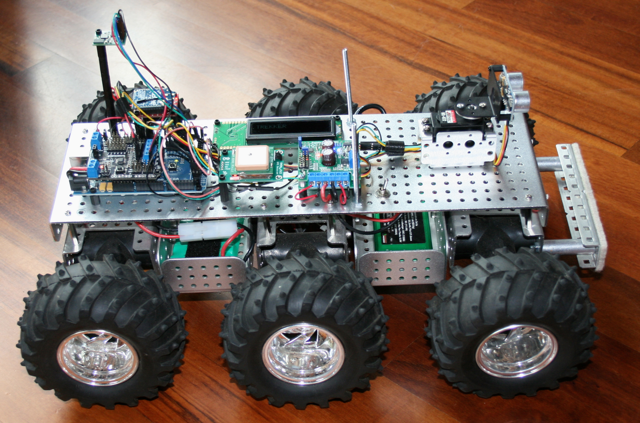
\includegraphics[height=7cm, keepaspectratio]{img/wheels.png}    
    \caption{Primer platforme sa šest točkova}
    \label{fig:wheels}
\end{figure}

\subsubsection{Gusenice}

Kretanje pomoću gusenica rešava neke od problema sa kojima se suočavaju platforme pokretane pomoću točkova. Konstantni kontakt gusenica sa tlom sprečava proklizavanje platforme. Pored ovoga, postojanje gusenica bolje raspoređuje težinu platforme, pa omogućava kretanje po površinama koje bi bile nepristupačne platformama zasnovanim na točkovima (npr. kretanje po snegu, pesku ili blatu), što je ilustrovano na slici \ref{fig:tracks}. Nedostaci ovakvog tipa kretanja su povećanje mehaničke kompleksnosti sistema i mali broj dostupnih gotovih gusenica, što ograničava prilagođavanje platforme korisniku. Takođe, ukoliko je robot težak, gusenice mogu oštetiti platformu po kojoj se kreću, što može predstavljati problem ako se robot kreće u zatvorenom prostoru.

\begin{figure}[H]
    \centering
    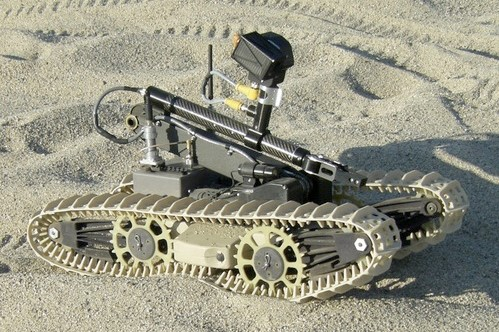
\includegraphics[height=7cm, keepaspectratio]{img/tracks.jpg}    
    \caption{Primer robota sa gusenicama, koji se kreće po pesku}
    \label{fig:tracks}
\end{figure}

\subsubsection{Noge}

Roboti sa nogama predstavljaju najsloženiji način kretanja zemljanih platformi. Postojanje nogu ne podrazumeva samo čovekoliko, bipedalno kretanje, već uključuje i kretanje sa četiri ili šest nogu. Roboti sa tri ili više nogu su mnogo jednostavniji za kontrolu od bipedalnih, budući da lakše održavaju ravnotežu. Ovakve platforme mogu zaobići veliki broj objekata koji im se mogu naći na putu, koje bi prethodno navedenim platformama predstavljale nepremostivu prepreku, pa su dobar izbor za vrlo grube terene. Uprkos ovome, roboti sa nogama zahtevaju veliku mehaničku, elektroničku i programsku složenost. Takođe cena izgradnje ovakvih robota je viša zbog velikog broja potrebnih delova. Primer robota sa četiri noge prikazan je na slici \ref{fig:legs}.

\begin{figure}[H]
    \centering    
    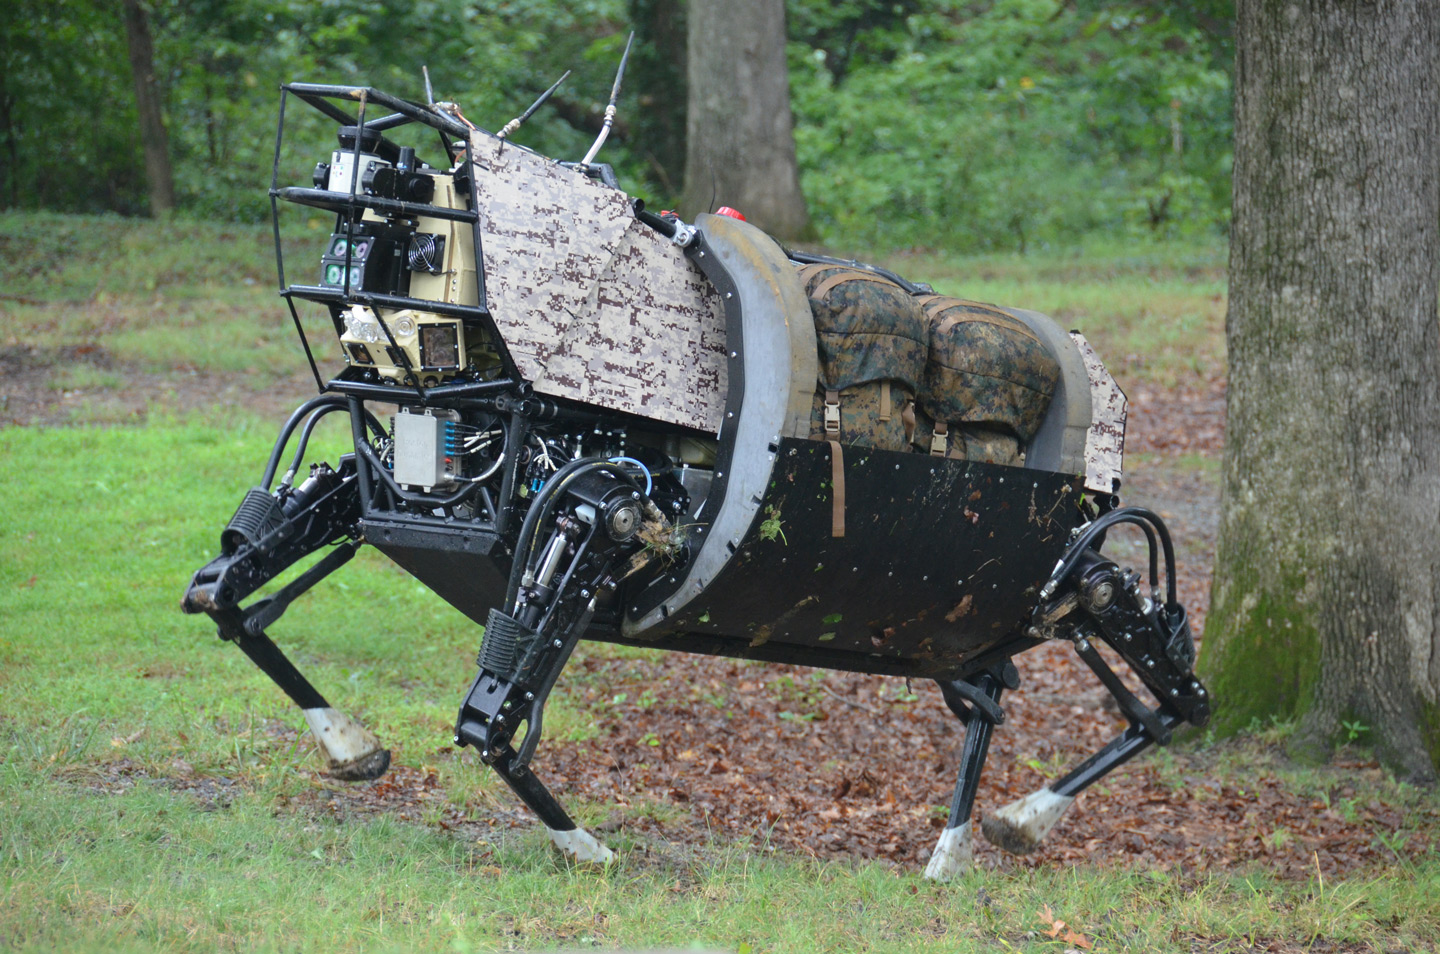
\includegraphics[height=7cm, keepaspectratio]{img/legs.jpg}    
    \caption{Primer napredne platforme sa četiri noge}   
    \label{fig:legs}
\end{figure}

\section{Komunikacija korisnika sa platformom}
U ovom odeljku su opisani najzastupljeniji vidovi komunikacije između platforme i udaljenog operatera \cite{communication-types}.

\subsubsection{Žičana}

Kontrola pomoću žice predstavlja najjednostavniji vid udaljene kontrole platforme. Jedna od prednosti žičane komunikacije je mogućnost napajanja robota preko žice, čime se eliminiše potreba za baterijama. Takođe, ovaj vid komunikacije je vrlo jednostavan, a prenos informacija preko žice je pouzdaniji od bilo kakvog bežičnog prenosa. Sa druge strane, maksimalna udaljenost platforme od operatera je ograničena dužinom žice, a žica se može zapetljati ili čak i prekinuti, čime bi se onemogućila dalja komunikacija sa robotom.   

\subsubsection{Radio komunikacija}

Radio komunikacija predstavlja najjednostavniji tip bežične kontrole platforme. Ovakav tip komunikacije se koristi u maketama automobila i aviona na daljinsko upravljanje. Radio komunikacija obezbeđuje kontrolu platformi na veoma velikim udaljenostima, što je čini vrlo pogodnom za korišćenje. Glavni nedostatak ovog tipa bežične komunikacije jeste vrlo mala brzina prenosa podataka u odnosu na druge vidove bežične komunikacije. Takođe, može doći do interferencije signala ukoliko više korisnika komunicira sa svojim uređajima na istoj frekvenciji.

\subsubsection{Bluetooth}

Komunikacija Bluetooth protokolom rešava neke od problema koji se javljaju kod razmene informacija putem jednostavne radio komunikacije. Bluetooth protokol zahteva direktno uparivanje dva uređaja, čime se izbegava interferencija sa drugim korisnicima. Takođe, Bluetooth omogućava veću brzinu prenosa podataka, ali po ceni drastično smanjene udaljenosti komunikacije, koja ovim protokolom iznosi maksimalno 10 metara.

\subsubsection{Wi-Fi}

Komunikacija putem Wi-Fi tehnologije zahteva postojanje bežične lokalne mreže na koji su povezani korisnik i platforma. Ovaj vid bežične komunikacije je nešto složeniji od prethodnih, budući da pri podešavanju zahteva dodatni programerski napor. Maksimalna udaljenost platforme i korisnika zavisi od jačine odašiljača bežične mreže, a ukoliko se iskoristi već postojeća mrežna infrastruktura korisnik može sa bilo koje tačke na svetu putem Internet protokola kontrolisati platformu koja je u dometu nekog odašiljača. Takođe, uz izbor odgovarajućeg odašiljača signala, Wi-Fi pruža najveće brzine prenosa podataka u poređenju sa ostalim vidovima bežične komunikacije.

\newpage

\section{Načini upravljanja}

\subsubsection{Ručni kontroleri}

Pod terminom ,,ručni kontroler'' podrazumeva se uređaj koji sadrži tastere, prekidače ili palice, koji služe za upravljanje udaljenom robotskom platformom. Ovo predstavlja najstariji način udaljenog upravljanja, i uključuje uređaje kao što su radio transmiteri i džojstici. Takođe ručni kontroleri mogu biti i upravljači iz konzola za video igre koji se pored svoje osnovne namene, mogu iskoristiti za jednostavnu kontrolu robotske platforme. Svi ovi kontroleri omogućavaju vrlo preciznu i intuitivnu kontrolu platforme, ali se pri dizajniranju same platforme i odabiru kontrolera mora paziti da se sve komande koje platforma može primiti mapiraju na kontroler, kako bi udaljena kontrola bila moguća.

\subsubsection{Miš i tastatura}

Kontrola pomoću miša i tastature, za razliku od ručnih kontrolera, zahteva postojanje personalnog računara kao posrednika u komunikaciji. Na računaru obično postoji interfejs koji tumači unos od strane miša i tastature i prosleđuje ih platformi. Uz dobro realizovan interfejs, ovakav vid kontrole omogućava izdavanje mnogo većeg broja komandi od ručnih kontrolera, ali je preciznost kontrole obično smanjena.

\subsubsection{Ostali načini upravljanja}
Prethodni načini upravljanja postoje već decenijama. Međutim, razvojem tehnologije mogući vidovi interakcije čoveka sa računarima su se drastično povećale. Samim tim, metode upravljanja robotskim platformama su takođe mnogobrojnije. U nastavku će biti dato nekoliko primera novijih načina kontrole robotskih platformi.

\textit{Leap Motion} je uređaj koji uz pomoć niza senzora omogućava prepoznavanje položaja šake i pokreta prstiju bez fizičkog kontakta \cite{leap}. Uređaj se sastoji od dve monohromatske infracrvene kamere i tri infracrvene svetleće diode, koje osvetljavaju prostor ispred uređaja. Uređaj prepoznaje svetlost odbijenu o šake i šalje te informacije na dalju obradu. Pomoću \textit{Leap Motion}-a se može pratiti položaj ruke i šake korisnika, koji robotska ruka potom imitira \cite{leap-article}.

\textit{Kinect} uređaj je razvila kompanija Microsoft kao dodatak za njihove \textit{Xbox} konzole za video igre \cite{kinect}. Ovaj uređaj pomoću kamera i infracrvenih senzora prepoznaje pokrete korisnika u prostoru, čime se omogućuje korisniku da pomeranjem ruku ili celog tela interaguje sa računarom. Kompanije i istraživači koji razvijaju humanoidne robote obično koriste \textit{Kinect} za preslikavanje pokreta upravljača na pokrete robota \cite{kinect-article}.

Jedan od novih načina interakcije sa računarima predstavlja tumačenje električnih impulsa koji proizvode mišići ruke. Jedan uređaj koji je zasnovan na tom principu je i \textit{Myo}, razvijen u kompaniji Thalmic Labs \cite{myo-specs}, koji će biti detaljnije opisan u narednom poglavlju. 

\newpage

\chapter{Projekat}
\section{Funkcionalna specifikacija}

U ovom odeljku je opisan način korišćenja sistema za udaljeno upravljanje robotskom platformom. Prvo je navedeno od kojih komponenti se sastoji ceo sistem, a zatim je opisano pokretanje celog sistema kao i interakcija korisnika sa prethodno pokrenutim sistemom.

Sistem se, na najvišem nivou, sastoji iz robotske platforme i veb prezentacije preko koje se korisniku omogućava kontrola ove platforme. Platformu, pored mehaničkih komponenti sačinjavaju i dva procesirajuća elementa: Raspberry Pi računar \cite{pi}, koji tumači komande primljene od korisnika i izdaje naredbe drugom procesirajućem elementu - mikrokontroleru koji se nalazi na Arduino platformi \cite{arduino}. Ovaj mikrokontroler interaguje sa svim mehaničkim komponentama platforme. Detaljnija arhitektura sistema biće data u odeljku \ref{sec:architecture}. 

Pomeranjem prekidača struja iz baterije počinje da napaja Raspberry Pi, čime sistem postaje spreman za rad. Raspberry Pi će pri pokretanju pokušati da se poveže na neku od prethodno zapamćenih bežičnih mreža. Ukoliko nijedna bežična mreža nije dostupna, Raspberry Pi se mora povezati Ethernet kablom na neku žičanu mrežu i tako konfigurisati za povezivanje na bežičnu. Drugi način za povezivanje je pristupanje grafičkom korisničkom interfejsu putem HDMI kabla, i konfigurisanje parametara za konekciju sa bežičnom mrežom. Na slici \ref{fig:myobot} je prikazan izgled konstruisane robotske platforme. Na prednjem delu platforme se nalaze kamera, četri svetleće diode i senzor udaljenosti. Na levoj i desnoj strani prednjeg dela platforme se nalaze motori i točkovi. U centralnom delu platforme, na levoj strani slike se nalazi Arduino platforma (u plavom kućištu), a sa desne Raspberry Pi.

\begin{figure}[H]
    \centering
    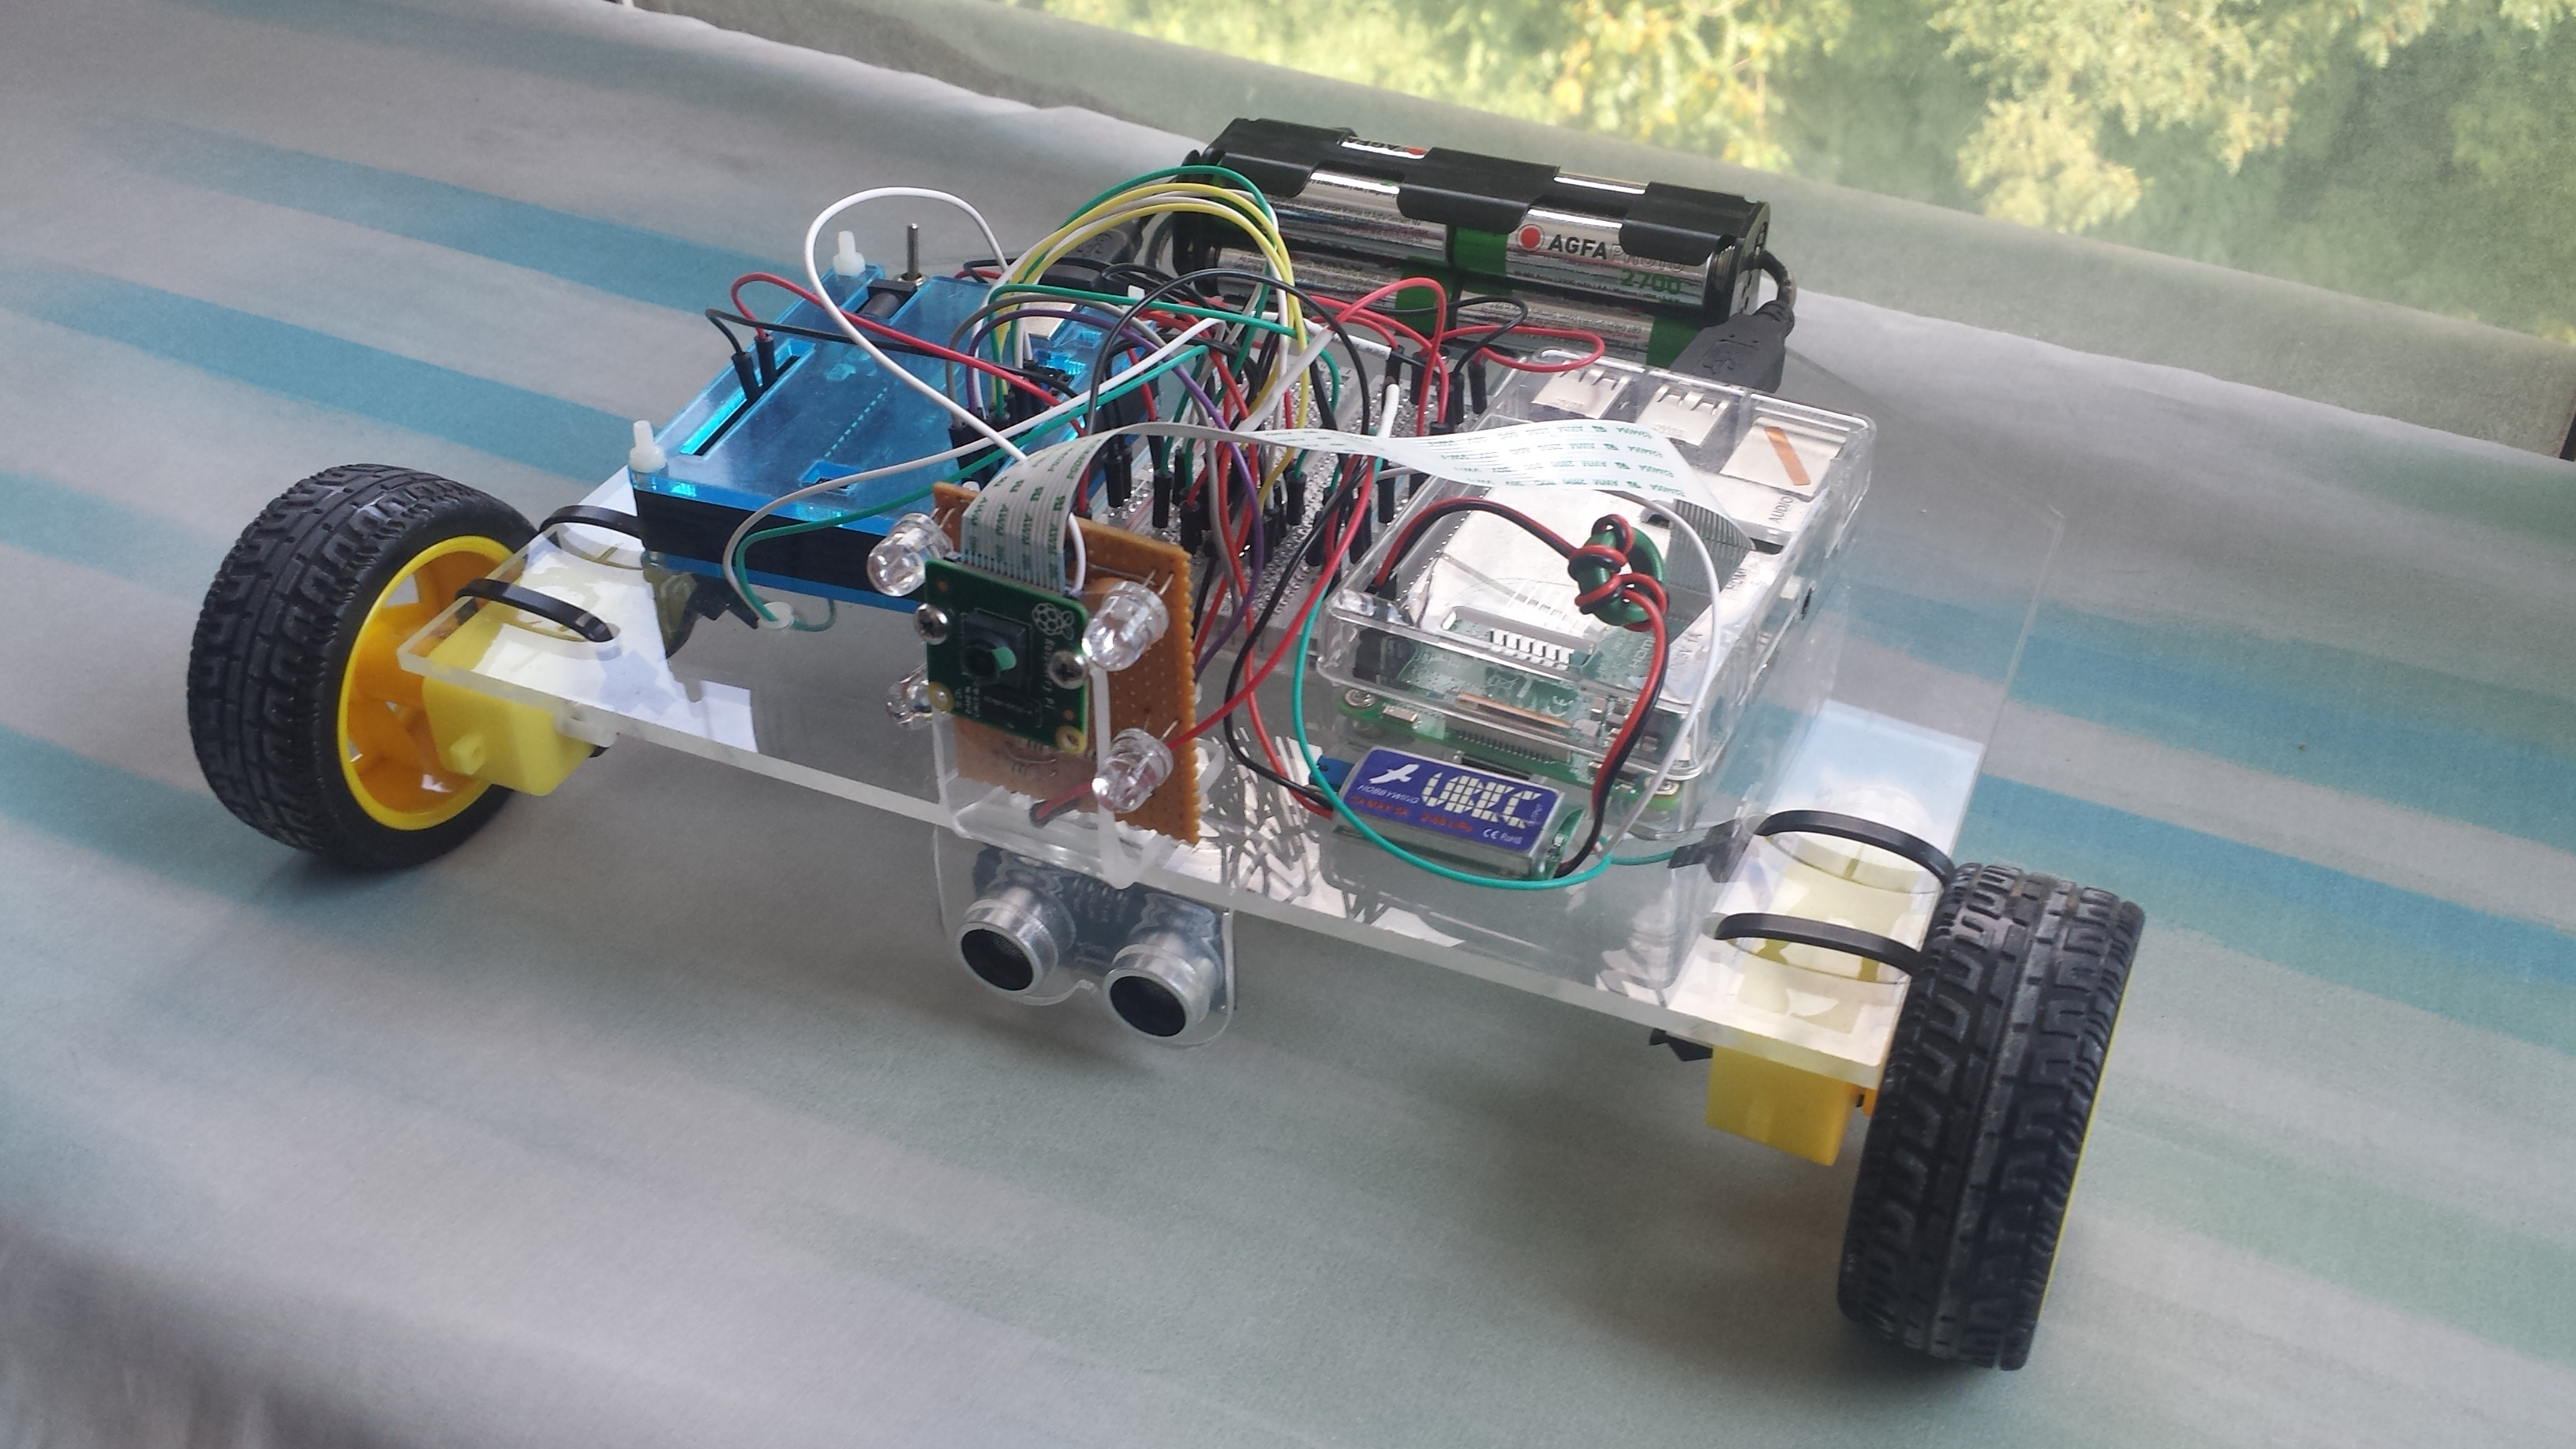
\includegraphics[width=16cm, keepaspectratio]{img/myobot.jpg}
    \caption{Prikaz ugašene platforme konstruisane za potrebe ovog rada}
    \label{fig:myobot}
\end{figure}

Nakon povezivanja na bežičnu mrežu, sistemu se mora pristupiti putem SSH ili VNC protokola, čime se dobija pristup konzoli ili grafičkom korisničkom interfejsu Raspberry Pi-a.

Zatim je potrebno doći do \texttt{home} direktorijuma ulogovanog korisnika, gde se nalazi Myobot direktorijum, koji predstavlja koreni direktorijum sistema za upravljanje platformom. U korenom direktorijumu se nalazi skripta \texttt{start.sh}, čijim izvršavanjem se pokreće server koji omogućava pristup sistemu za udaljeno upravljanje ovom platformom. Slika \ref{fig:putty} prikazuje logovanje na Raspberry Pi računar putem SSH protokola, korišćenjem PuTTY alata, i naknadno pokretanje servera.

\begin{figure}[H]
    \centering
    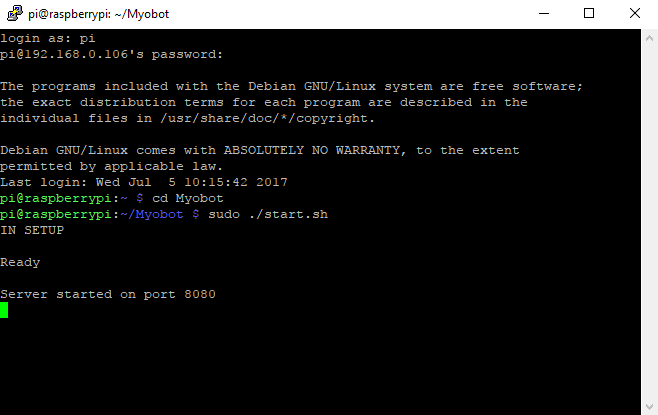
\includegraphics[width=16cm, keepaspectratio]{img/putty.png}
    \caption{Prikaz logovanja na Raspberry Pi i pokretanja sistema}
    \label{fig:putty}
\end{figure}

U okviru korisnikovog veb pregledača potrebno je uneti adresu povezanog Raspberry Pi-a, kao i port na kome je pokrenut server. Dolaskom na ovu adresu korisniku se prikazuje veb prezentacija sistema. Na slici \ref{fig:index_with_sidebars} je prikazana početna stranica korisničkog interfejsa za udaljenu kontrolu platforme. Prikaz slike je isključen, a pomoćni meni i meni sa dodatnim komandama su otvoreni.

\begin{figure}[H]
    \centering
    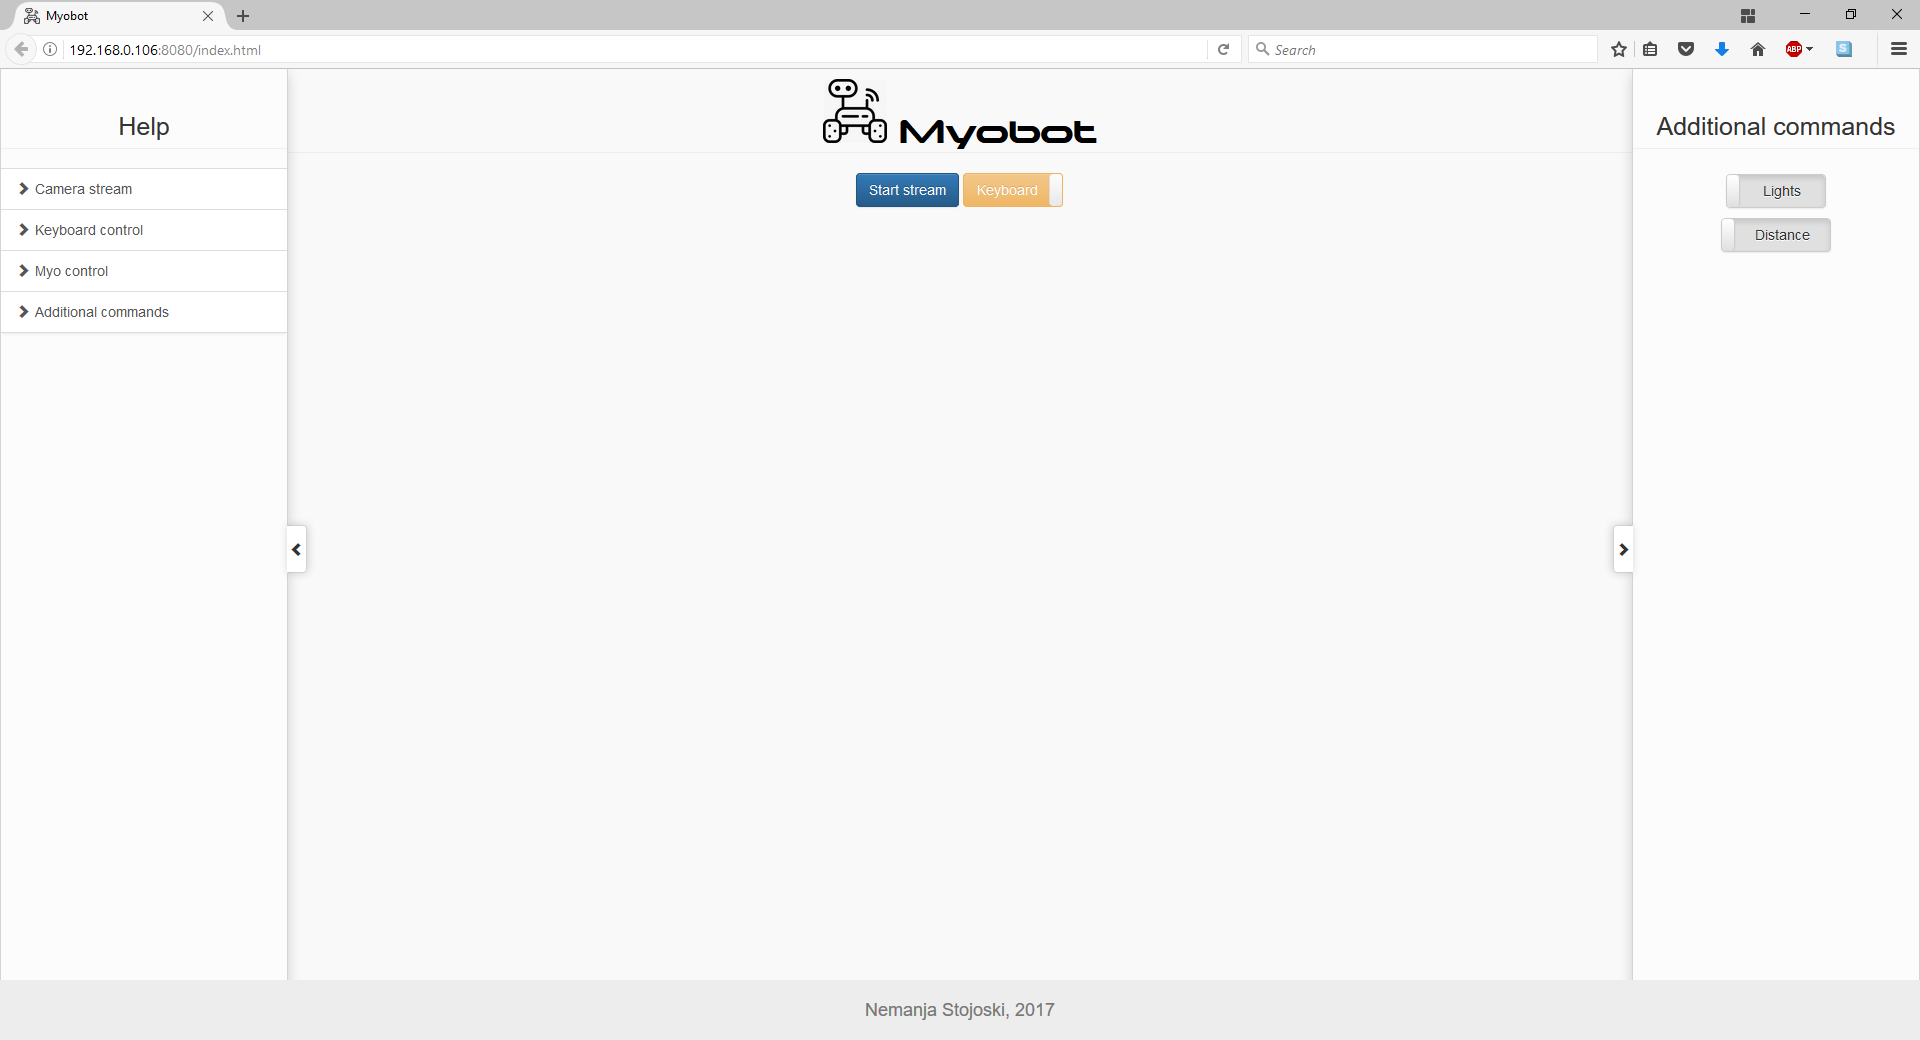
\includegraphics[width=16cm, keepaspectratio]{img/index_with_sidebars.png}
    \caption{Početna stranica korisničkog interfejsa}
    \label{fig:index_with_sidebars}
\end{figure}

Navedena veb prezentacija korisniku omogućava pristup kontrolama za upravljanje platformom. U bilo kom trenutku, korisnik može pokrenuti ili zaustaviti prenos slike sa kamere. Korisniku se takođe daje mogućnost odabira načina kontrole platforme. Podrazumevan način kontrole je pomoću tastature. Ukoliko korisnik poseduje \textit{Myo} narukvicu i na svom računaru ima instaliran Myo Connect program za povezivanje sa narukvicom, nakon stavljanja narukvice i njene sinhronizacije sa Myo Connect programom korisniku se omogućava kontrola platforme pomoću narukvice. Ukoliko korisnik odabere ovaj način kontrole platforme, zahtevi za pokretanjem platforme šalju se pravljenjem predefinisanih pokreta šake. 

Pored prenosa slike i kontrole platforme, korisniku je dostupan meni sa dodatnim opcijama, koji se nalazi na desnoj strani prezentacije. U tom meniju korisnik ima mogućnost da od platforme zatraži trenutno izmerenu udaljenost od prepreke koja se može nalazititi ispred platforme. Merenje je podešeno tako da vraća udaljenosti do 1 m. Takođe, korisnik može upaliti ili ugasiti svetla na platformi, čime se omogućava rad platforme u mračnim područjima.

Na levoj strani prezentacije korisniku je dostupan pomoćni meni koji objašnjava mogućnosti platforme i služi kao uputstvo za korišćenje sistema. Slika \ref{fig:cats} prikazuje korisnički interfejs sa uključenim prikazom slike sa kamere i aktiviranim svetlećim diodama, za rad u slabo osvetljenom okruženju.

\begin{figure}[H]
    \centering
    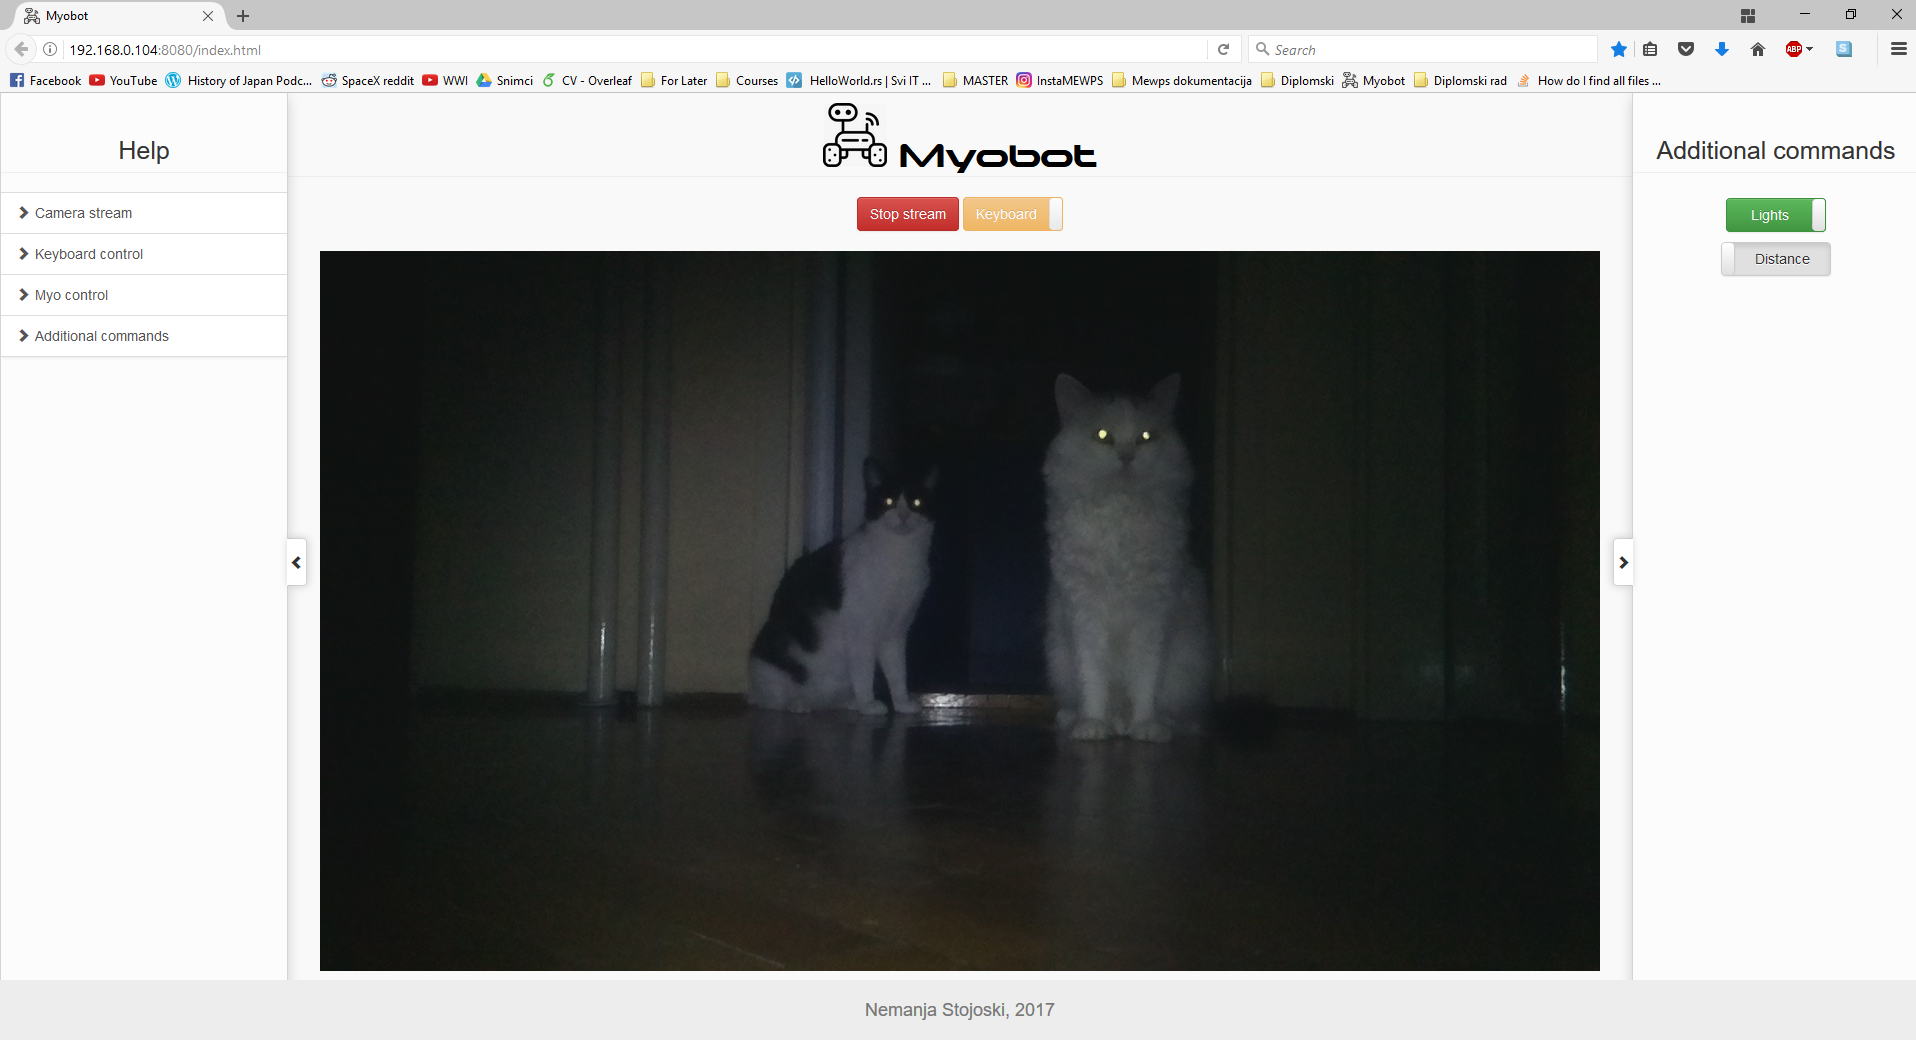
\includegraphics[width=16cm, keepaspectratio]{img/cats.png}
    \caption{Prikaz rada u slabo osvetljenom okruženju, na primeru Baleriona i Garfilda}
    \label{fig:cats}
\end{figure}

\section{Arhitektura sistema} \label{sec:architecture}
U ovom odeljku je opisana detaljna arhitektura hardverske i softverske celine projekta.
\subsection{Arhitektura hardvera}
\subsubsection{Raspberry Pi}
Raspberry Pi je ,,single-board''\footnote{,,single-board'' računar: Računar malih dimenzija kod kojeg su sve komponente potrebne za rad računara zalemljene za jednu ploču.} računar zasnovan na 64-bitnom ARMv8 procesoru \cite{pi}. Za potrebe ovog rada, na njega je instaliran Raspbian operativni sistem. Raspbian je operativni sistem zasnovan na Linux Debian operativnom sistemu i optimizovan za hardver Raspberry Pi-a \cite{raspbian}. Korišćena verzija ovog računara je Raspberry Pi 3 Model B, koja je izabrana zato što poseduje bežičnu lokalnu mrežnu konekciju (Wi-Fi), koja je potrebna radi udaljenog povezivanja sa robotskom platformom. U ovom projektu, Raspberry Pi ima dve svrhe: funkcioniše kao server koji opslužuje korisnika povezanog preko lokalne mreže, i na osnovu zahteva primljenih od korisnika izdaje komande Arduino mikrokontrolerskoj platformi.
\subsubsection{Arduino}
Arduino je mikrokontrolerska platforma otvorenog hardvera i otvorenog koda koja služi za razvoj elektronskih projekata. Korišćena verzija ove platforme je Arduino Uno Rev3, zasnovana na Atmel ATmega328P mikrokontroleru \cite{arduino}. Odabrana je za izradu ovog projekta zbog jednostavnosti programiranja, kompatibilnosti sa velikim brojem senzora kao i dostupnosti obimne dokumentacije. Sadrži 14 digitalnih input/output pinova, od kojih 6 mogu da se koriste kao PWM\footnote{PWM: Pulse Width Modulation - Modulacija širine pulsa; u ovom projektu PWM pinovi se koriste kako bi se mogle podesiti različite brzine obrtaja motora: brzom aktivacijom i gašenjem kvadratnih talasa različitog trajanja, stiče se privid menjanja napona koji izlazi iz PWM pina, od 0V do 5V.} output pinovi, kao i 6 analognih input pinova. Ovi pinovi se koriste u projektu za povezivanje sa senzorima i drugim komponentama. Arduino i Raspberry Pi su povezani USB kablom koji omogućava njihovu međusobnu komunikaciju, kao i napajanje Arduno-a strujom napona od 5V. Kod za Arduino platformu može da se piše u jezicima C i C++, uz poštovanje određenih pravila za strukturiranje koda.
\subsubsection{Senzor udaljenosti}
U ovom projektu je korišćen HC-SR04 ultrazvučni senzor udaljenosti  \cite{distance}. Pored standardnih pinova za napajanje, ovaj ultrazvučni senzor poseduje \emph{Trigger} pin za slanje ultrazvučnog talasa, kao i \emph{Echo} pin koji se gasi kada senzor primi odbijeni talas. Princip funkcionisanja je sledeći: \emph{Trigger} pin se drži aktivnim najmanje 10 mikrosekundi nakon čega senzor emituje 8 kratkih ultrazvučnih pulseva frekvencije 40 kHz i aktivira \emph{Echo} pin. Ovaj pin se gasi kada senzor registruje odbijeni ultrazvučni talas, pa se, poznajući brzinu prostiranja mehaničkih talasa u vazduhu na određenoj temperaturi kao i dužinom trajanja aktivne vrednosti na \emph{Echo} pinu može proceniti udaljenost objekta o koji su se odbili ultrazvučni talasi. Preciznost ovog senzora je do 3 mm, a može detektovati objekte udaljene od 2 cm do 400 cm.
\subsubsection{Ostale komponente na platformi}
Za pokretanje robotske platforme korišćena su dva DC motora sa reduktorom obrtaja, čiji je preporučeni radni napod od 3 V do 12 V. Za pokretanje motora je korišćen L293D čip koji se sastoji od dva H-mosta\footnote{H-most - Električno kolo koje omogućava primenu napona na potrošača u različitim smerovima; u ovom projektu, H-mostovi u L293D čipu se koriste da bi motori mogli da se kreću unapred ili unazad. Postavljanjem napona na jedan pin L293D čipa motor će se okretati u jednom smeru, dok će se postavljanjem napona na drugi pin čipa motor okretati u suprotnom smeru.}, koji omogućavaju istovremeno kontrolisanje oba motora od strane Arduino-a \cite{l293d}.

Motore platforme i Raspberry Pi napaja 8 redno vezanih punjivih Ni-Mh AA baterija kapaciteta 2300 mAh. Svaka baterija je napona 1.2 V, pa je ukupni napon 9.6 V. Budući da Raspberry Pi zahteva napon od 5 V, mora se koristiti neka vrsta reduktora napona da bi sistem ispravno funkcionisao. Za to je iskorišćen UBEC (Universal Battery Elimination Circuit): uređaj koji smanjuje napon sa baterija (sa maksimalno 26 V) na potrebnih 5V \cite{ubec}. Maksimalna jačina struje koju pruža je 3 A, što je dovoljno za rad celokupne platforme.

Za snimanje videa u realnom vremenu, korišćena je Raspberry Pi Camera, povezana na CSI (Camera Serial Interface) port Raspberry Pi-a \cite{picamera}. Senzor ima rezoluciju od 8 megapiksela, i omogućava snimanje videa u 1920x1080 rezoluciji brzinom do 30 slika u sekundi.

Na platformi se takođe nalaze i četiri svetleće diode koje mogu služiti kao noćno svetlo, čime se platforma osposobljava za funkcionisanje u slabo osvetljenim područjima.

\subsubsection{Myo narukvica}
Kao jedan vid udaljene kontrole platforme korišćena je \textit{Myo} narukvica za prepoznavanje pokreta. Prepoznavanje pokreta na ovoj narukvici se zasniva na dva principa \cite{myo}. Prvi je elektromiografija tj. merenje električnog potencijala ćelija u mišićima ruke. Budući da svaki položaj šake proizvodi jedinstven električni ,,potpis'' u mišićima podlaktice, on se može prepoznati i zabeležiti određeni položaj šake. Drugi princip prepoznavanja pokreta zasniva se na određivanju orijentacije narukvice u prostoru, kao i njenog ubrzanja tokom vremena, čime se mogu prepoznati karakteristični pokreti cele ruke kao što je mahanje ili kruženje. Za potrebe ovog projekta korišćeno je samo prepoznavanje pokreta zasnovano na merenju električne aktivnosti mišića, uz prepoznavanje predefinisanih položaja šake. 

\subsubsection{Šeme povezivanja}
Ovde su date šeme povezivanja glavnih podsistema platforme: povezivanje Arduino-a sa senzorom udaljenosti, povezivanje sa motorima i baterijama, kao i podsistem za paljenje i gašenje svetlećih dioda.

Slika \ref{fig:distance_sensor} prikazuje povezivanje Arduino-a sa HC-SR04 ultrazvučnim senzorom. Crvene žice predstavljaju napon, crne uzemljenje, siva žica je povezana sa \textit{Trigger} pinom, a ljubičasta sa \textit{Echo} pinom.

\begin{figure}[H]
    \centering
    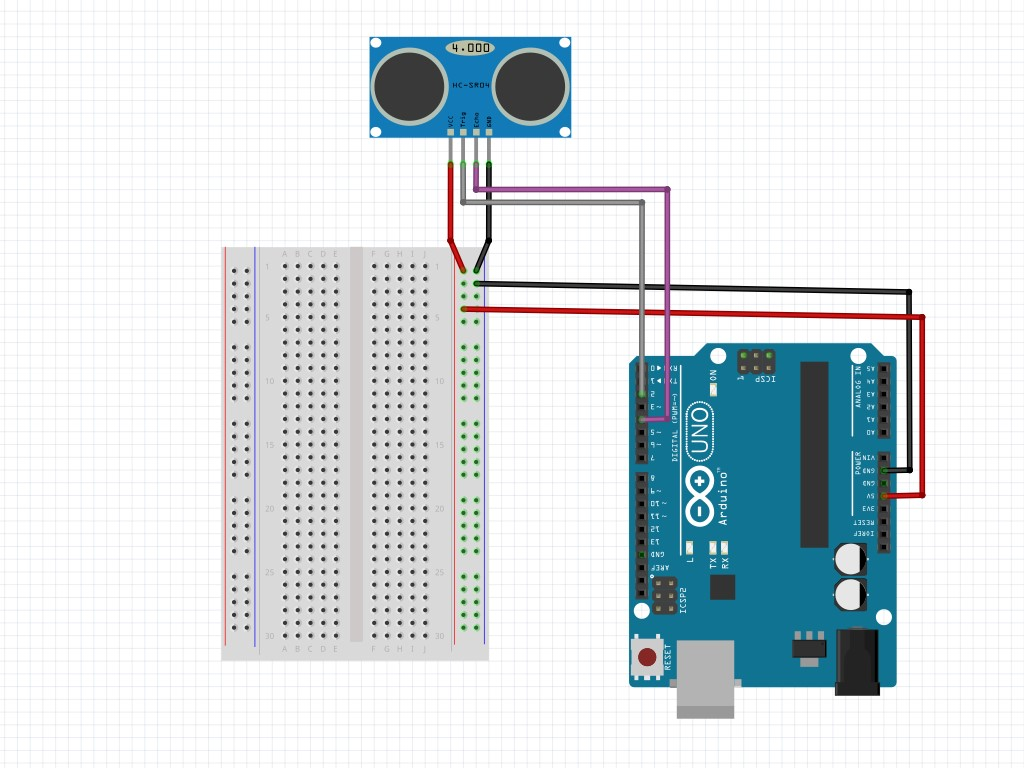
\includegraphics[scale=0.41]{img/distance_sensor.jpg}
    \caption{Povezivanje Arduino-a sa HC-SR04 ultrazvučnim senzorom.}
    \label{fig:distance_sensor}
\end{figure}

Na slici \ref{fig:motors} je prikazano povezivanje Arduino-a sa L293D čipom i njegovo povezivanje sa dva DC motora. Takođe je prikazano i dovođenje napona sa baterija i sa Arduino-a na odgovarajuce pinove L293D čipa. Crvene žice predstavljaju napon, crne uzemljenje, a ostale služe za povezivanje Arduino-a i čipa radi ispravne kontrole motora.

\begin{figure}[H]
    \centering
    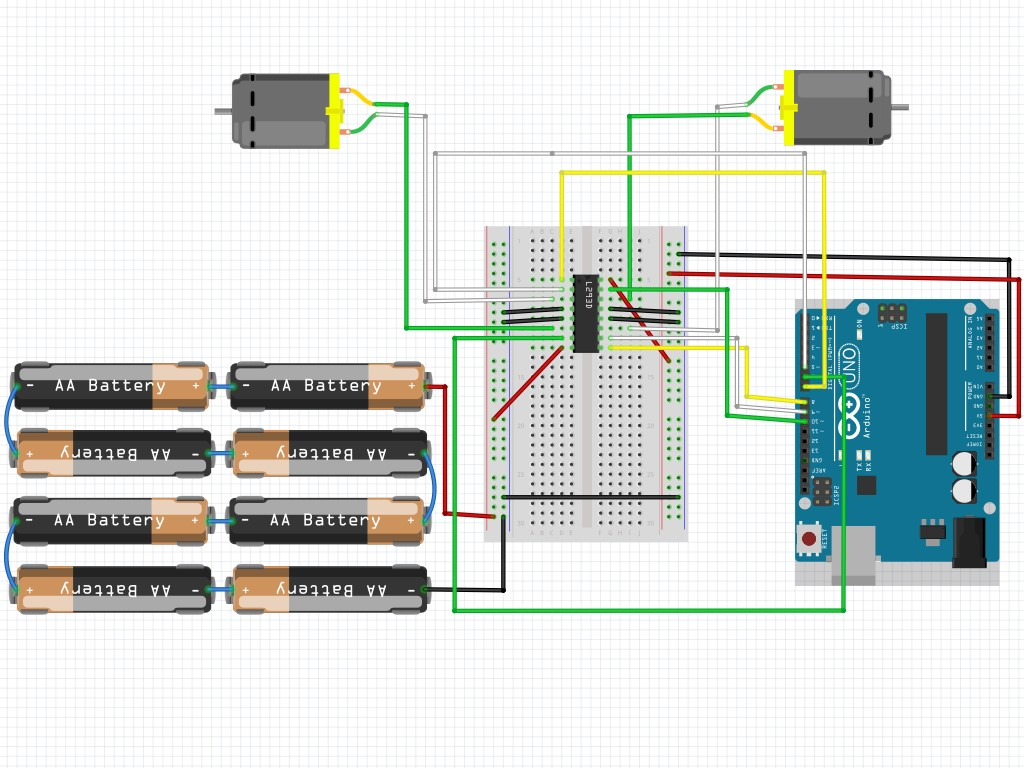
\includegraphics[scale=0.41]{img/motors.jpg}
    \caption{Podsistem za kretanje platforme.}
    \label{fig:motors}
\end{figure}

Na slici \ref{fig:lights} je prikazano povezivanje baterija i Arduino-a sa četiri svetleće diode. Paljenje i gašenje dioda kontroliše FQP30N06L MOSFET tranzistor \cite{mosfet}, koji u ovom kolu funkcioniše kao prekidač. Kada Arduino postavi napon sa svog pina 12 na \textit{Gate} pin tranzistora, on dozvoljava protok struje iz baterija kroz diode, čime se one aktiviraju. 

\begin{figure}[H]
    \centering
    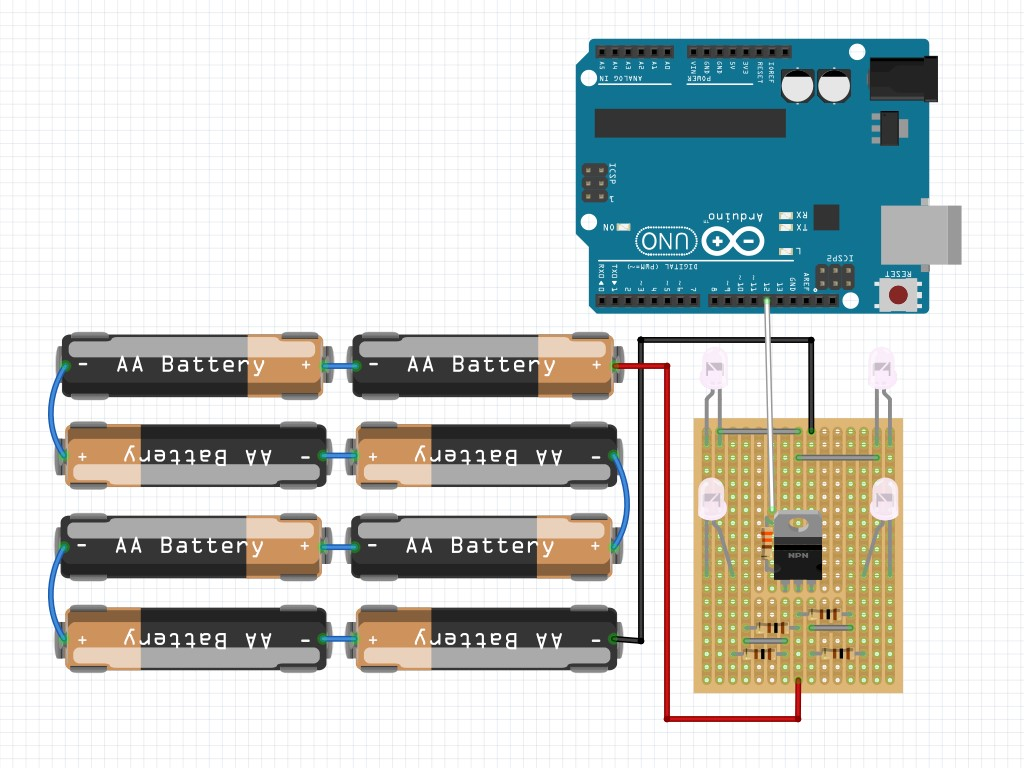
\includegraphics[scale=0.41]{img/lights.jpg}
    \caption{Povezivanje Arduino-a sa svetlećim diodama.}
    \label{fig:lights}
\end{figure}

\subsection{Arhitektura softvera}
Softver ovog sistema se sastoji iz tri celine: koda koji se izvršava na Arduino platformi, koda koji se izvršava na Raspberry Pi računaru i koda koji se izvršava na klijentskom uređaju. Nakon svakog odeljka priložena je struktura direktorijuma koja odgovara toj celini, sa ključnim fajlovima i poddirektorijumima. Slika \ref{fig:myobot_dir} prikazuje strukturu korenog direktorijuma projekta. U korenom direktorijumu se nalazi Bash skripta \texttt{start.sh} koja pokreće \texttt{main.py} fajl iz Pi direktorijuma. Ukoliko je ovoj skripti prenet opcioni argument ,,-u'', skripta će prevesti kod iz Arduino direktorijuma i učitati prevedeni kod na Arduino mikrokontroler. Skripta se mora pokrenuti od strane \texttt{root} korisnika komandom \texttt{sudo}, da bi se obezbedilo uspešno izvršavanje svih komandi u ovoj skripti, budući da neke od njih zahtevaju privilegije \texttt{root} korisnika.

\begin{figure}[H]
  \centering
  \begin{forest}
    pic dir tree,
    where level=0{}{% folder icons by default; override using file for file icons
      directory,
    },
    [Myobot
        [Arduino]
        [Pi]
        [Web]
        [start.sh, file]
    ]
  \end{forest}
  \caption{Struktura korenog direktorijuma projekta}
  \label{fig:myobot_dir}
\end{figure}
\newpage
\subsubsection{Arduino}
Kod na Arduino platformi se nalazi u jednom fajlu (\texttt{sketch.ino}). Pored pomoćnih funkcija, sadrži dve glavne funkcije koje moraju postojati u svakom programu koji se izvršava na Arduino platformi: \texttt{setup()} i \texttt{loop()}. Funkcija \texttt{setup()} se poziva jednom pri pokretanju Arduino uređaja, a zatim se funkcija \texttt{loop()} poziva neprekidno dok se Arduino ne ugasi ili se ne učita novi kod u njega. Slika \ref{fig:arduino_dir} prikazuje strukturu Arduino poddirektorijuma.

U \texttt{setup()} funkciji se inicijalizuju pinovi koji se koriste za interakciju sa senzorom udaljenosti, pinovi za kontrolu motora, kao i pin za aktivaciju svetlećih dioda. Takođe, ovde se inicijalizuje serijska komunikacija putem USB kabla sa Raspberry Pi-em, podešavanjem brzine prenosa podataka koja mora biti postavljena na istu vrednost na oba kraja komunikacije.

U \texttt{loop()} funkciji se ponavljaju tri glavne celine: Prva je periodična provera da li je potrebno aktivirati senzor udaljenosti. On se aktivira ukoliko je Arduino primio \texttt{START} komandu za početak rada, ukoliko se platforma kreće napred ili korisnik zahteva merenje udaljenosti, i ukoliko je prošlo dovoljno vremena od prethodnog merenja udaljenosti (nekoliko desetina milisekundi). Ukoliko su ovi uslovi ispunjeni, Arduino aktivira senzor i postavlja funkciju koja će se pozivati prekidom internog tajmera i proveravati da li je izmerena udaljenost od senzora. Zatim se proverava poslednje vreme stizanja \textit{heartbeat} signala od Raspberry Pi-a. Ukoliko novi signal ne stigne u određenom vremenskom roku to može značiti da je komunikacija između Raspberry Pi-a i Arduino-a na neki način kompromitovana. Motori u tom trenutku mogu biti uključeni, i ne menjaju svoje stanje dok ne stigne zahtev za njihovo gašenje. Ukoliko je komunikacija kompromitovana, zahtev možda nikad ne stigne, pa Arduino preventivno gasi motore da ne bi došlo do štete na platformi. Na kraju se proverava da li je stigla nova komanda od Raspberry Pi-a. O ovim komandama će biti više reči u delu rada posvećenom detaljima implementacije.

\begin{figure}[H]
  \centering
  \begin{forest}
    pic dir tree,
    where level=0{}{% folder icons by default; override using file for file icons
      directory,
    },
    [Arduino
        [lib
          [NewPing
              [NewPing.cpp, file]
              [NewPing.h, file]
          ]
        ]
        [src      	
          [sketch.ino, file]
        ]      
    ]
  \end{forest}
  \caption{Struktura Arduino poddirektorijuma}
  \label{fig:arduino_dir}
\end{figure}
\vspace{-5mm}
\subsubsection{Raspberry Pi}
Na Raspberry Pi-u se izvršava najveći deo koda potreban za funkcionisanje ovog sistema. Pi poddirektorijum se sastoji se od 8 fajlova napisanih u Python programskom jeziku i jednog konfiguracionog fajla, što je prikazano na slici \ref{fig:pi_dir}. U daljem tekstu sledi kratak opis funkcije svakog fajla. 

\begin{itemize}
\vspace{-1mm}
\item \texttt{config.ini}

Ovaj fajl sadrži konfiguracione parametre za Python kod koji se izvršava na Raspberry Pi-u. Ovde se nalaze parametri neophodni za povezivanje sa Arduinom (port za USB serijsku komunikaciju i brzina prenosa), parametri potrebni za pokretanje servera (port i dimenzije slike koja će prikazivati prenos sa kamere), kao i podešavanja za Raspberry Pi kameru (rezolucija, horizontalni i vertikalni obrt kamere).
\vspace{-1mm}
\item \texttt{shared.py}

Ovde se nalazi funkcija \texttt{init()} koja deklariše i definiše sve promenljive kojima se pristupa iz više fajlova. U ovoj fuknciji se takođe vrši i učitavanje parametara iz konfiguracionog fajla. Svi fajlovi kojima je potreban pristup globalnim promenljivama uključuju ovaj fajl kako bi mogli da pristupe tim promenljivama.
\vspace{-1mm}
\item \texttt{comm\_protocol.py}

U ovom fajlu se nalazi klasa \texttt{Communicator} koja služi za komunikaciju sa Arduino uređajem. Sem konstruktora, ova klasa sadrži metode \texttt{send()} i \texttt{receive()} koje se koriste za slanje i prijem podataka, respektivno. Metodu \texttt{send()} može pozivati više niti pa je potrebno zaštititi njen kod jednim \texttt{Lock} objektom.
\vspace{-1mm}
\item \texttt{serial\_receiver.py}

Ovde se nalazi klasa \texttt{SerialReceiver} čiji objekti predstavljaju zasebne niti izvršavanja programa. U njenoj \texttt{run()} metodi se tokom celog trajanja programa poziva \texttt{receive()} metoda iz prethodne klase, čime se čeka pristizanje vrednosti iz Arduino-a. Ukoliko ova metoda prepozna pristizanje informacije o izmerenoj udaljenosti, pomoću objekta klase \texttt{Event} obaveštava nit koja potencijalno čeka da pročita ovu informaciju da je ona stigla.
\vspace{-1mm}
\item \texttt{heartbeat.py}

Ovaj fajl sadrži klasu \texttt{Heartbeat} čiji objekti predstavljaju zasebne niti izvršavanja programa. U njenoj \texttt{run()} metodi se tokom celog trajanja programa šalje \textit{heartbeat} signal nakon isteka određenog vremenskog intervala.
\vspace{-1mm}
\item \texttt{hardware.py}

U ovom fajlu se nalaze tri klase, \texttt{Distance}, \texttt{Motors} i \texttt{Lights}, koje predstavljaju interfejs za slanje zahteva Arduino platformi, koja potom interaguje sa hardverom na željeni način.

Klasa \texttt{Distance} sadrži metode \texttt{distance\_on()} i \texttt{distance\_off()} koje signaliziraju Ar\-duino-u da započne ili zaustavi merenje udaljenosti na korisnički zahtev. Ovde se nalazi i metoda \texttt{get\_distance()} koja traži od Arduino-a poslednju udaljenost izmerenu ultrazvučnim senzorom. Ova metoda se blokira na \texttt{Event} objektu, kojem \texttt{SerialReceiver} nit signalizira da se može nastaviti sa radom, kada pristigne izmerena udaljenost.

Klasa \texttt{Motors} sadrži metode za pokretanje motora platforme. Ključna metoda u ovoj klasi je \texttt{set\_motor\_powers()} koja prima dva parametra koji predstavljaju procentualnu jačinu željene aktivacije motora. Ukoliko su prosleđeni parametri u odgovarajućem opsegu ona šalje Arduino-u komandu za pokretanje motora, zajedno sa zahtevanom jačinom aktivacije motora. Pored ove metode, ovde se nalazi i metoda \texttt{go()} koja pored istih parametara kao i prethodna metoda prima i opcione parametre \texttt{stop} i \texttt{duration} (koji su podrazumevano postavljeni na \texttt{False} i \texttt{1}, respektivno). Metoda \texttt{go()} prvo poziva metodu \texttt{set\_motor\_powers()} i prosleđuje joj svoje parametre za aktivaciju motora. Dodatno, ukoliko je \texttt{stop} parametar postavljen na \texttt{True}, ova metoda uspavljuje pozivajuću nit onoliko vremena koliko je prosleđeno \texttt{duration} parametrom i nakon toga zaustavlja motore. Ostale metode u ovoj klasi pozivaju metodu \texttt{go()} prosleđujući joj potrebne vrednosti radi zaustavljanja platforme, kretanja napred, nazad, skretanja levo ili skretanja desno.

Klasa \texttt{Lights} sadrži metode \texttt{lights\_on()} i \texttt{lights\_off()} koje šalju odgovarajuće zahteve Arduino-u za paljenje i gašenje svetlećih dioda na platformi.
\vspace{-1mm}
\item \texttt{server.py}

U ovom fajlu se nalaze sve klase potrebne za uspostavljanje servera na lokalnoj mreži. Objekti Klase \texttt{StreamingOutput} sadrže bafer za primanje nove slike sa kamere, najskoriju primljenu sliku, kao i objekat klase \texttt{Condition} koji služi za sinhronizovanje ,,proizvođača'' slika - kamere i ,,potrošača'' slika - klijenta koji šalje zahtev za novom slikom. Klasa \texttt{StreamingHandler} predstavlja osluškivač HTTP POST i GET zahteva. POST zahtevi predstavljaju zahteve poslate od strane klijenta AJAX protokolom, a GET zahtevi predstavljaju zahteve za novim HTML, CSS ili JavaScript stranicama, kao i zahteve za novom slikom sa kamere. Klasa \texttt{StreamingServer} je izvedena iz klase \texttt{server.HTTPServer} uz podešavanje da obrađuje svaki pristigli zahtev u zasebnoj niti. Pri konstrukciji, njoj se prosleđuje prethodno napravljeni \texttt{StreamingHandler} kao rukovalac zahtevima.
\vspace{-1mm}
\item \texttt{command\_executor.py}

U ovom fajlu se nalazi klasa \texttt{CommandExecutor} sa metodom \texttt{interpret()} koja izvršava zahteve tumačeći poruku primljenu od klijenta AJAX protokolom. To mogu biti zahtevi za pokretanje ili zaustavljanje platforme, pokretanje ili zaustavljanje prenosa sa kamere, zahtev za dohvatanje najnovije vrednosti izmerene senzorom udaljenosti kao i zahtevi za paljenje ili gašenje svetla na platformi. Ovde se takođe nalazi i asocijativni niz parova ključeva i vrednosti, gde ključevima odgovaraju poruke dobijene od klijenta a vrednostima imena metoda koje trebaju da se izvrše primanjem odgovarajuće poruke. Ovo je urađeno da bi se ubrzalo izvršavanje komandi i uprostio kod izbegavanjem dugačkih \texttt{if/elif} konstrukcija.
\vspace{-1mm}
\item \texttt{main.py}

Ovde se nalazi glavna funkcija, \texttt{main()} koja se izvršava pri pozivu skripte za pokretanje sistema. U njoj se prvo poziva funkcija \texttt{init()} iz \texttt{shared.py} fajla, koja inicijalizuje sve deljene globalne promenljive. Nakon ovoga se pokreće nit za prihvatanje vrednosti sa Arduino-a (\texttt{SerialReceiver}) kao i nit za održavanje \textit {heartbeat} signala (\texttt{Heartbeat}). Zatim se Arduino-u šalje komanda za početak komunikacije, i pokreće server (\texttt{StreamingServer}) koji osluškuje zahteve klijenata. Kada korisnik prekine izvršavanje programa šalje se signal prethodno pokrenutim nitima da prestanu sa izvršavanjem, čime se zaustavlja ceo program.

\end{itemize}

\begin{figure}[H]
  \centering
  \begin{forest}
    pic dir tree,
    where level=0{}{% folder icons by default; override using file for file icons
      directory,
    },
    [Pi
        [comm\_protocol.py, file]
        [command\_executor.py, file]
        [config.ini, file]
        [heartbeat.py, file]
        [main.py, file]
        [hardware.py, file]
        [serial\_receiver.py, file]
        [server.py, file]
        [shared.py, file]
    ]
  \end{forest}
  \caption{Struktura Pi poddirektorijuma}
  \label{fig:pi_dir}
\end{figure}

\subsubsection{Web}

Ovde se nalazi kod koji server šalje klijentu i koji se potom izvršava na klijentskom uređaju. Pored početne HTML stranice, \texttt{index.html}, i fajlova koji služe za stilizovanje veb prezentacije, ovde se nalazi i JavaScript fajl \texttt{myscript.js} koji sadrži funkcije potrebne za komunikaciju klijenta i servera AJAX protokolom kao i osluškivače događaja sa miša, tastature ili \textit{Myo} narukvice, koji generišu AJAX zahteve. Pri kontroli tastaturom, pritiskom određenog slova generiše se AJAX zahtev za pokretanje motora. Pri otpuštanju tog slova generiše se zahtev za zaustavljanjem motora. Slično, pri kontroli pomoću \textit{Myo} narukvice, kada se prepozna određeni pokret ruke šalje se AJAX zahtev za pokretanje motora, dok se prepoznavanjem prekida određenog pokreta šalje zahtev za zaustavljanjem motora. Takođe, pritiskom na odgovarajuću dugmad ili pravljenjem odgovarajućih pokreta ruke se šalju zahtevi za najskorijom vrednošću izmerenom senzorom udaljenosti, kao i zahtevi za paljenjem i gašenjem svetla na platformi. Slika \ref{fig:web_dir} prikazuje strukturu Web poddirektorijuma.

\begin{figure}[H]
  \centering
  \begin{forest}
    pic dir tree,
    where level=0{}{% folder icons by default; override using file for file icons
      directory,
    },
    [Web
        [css
          [..., file]
        ]
        [fonts
          [..., file]
        ]
        [js
          [..., file]
          [myo.js, file]
          [myscript.js, file]
        ]
        [..., file]
        [index.html, file]
    ]
  \end{forest}
  \caption{Struktura Web poddirektorijuma}
  \label{fig:web_dir}
\end{figure}

\section{Detalji implementacije}

U ovom odeljku su detaljnije opisani neki karakteristični delovi sistema.

\subsubsection{Komande za Arduino}
 Komande koje Arduino može primiti od Raspberry Pi-a su:
 
 \begin{itemize}
\vspace{-1mm}
\item \texttt{START} - Ovu komandu Raspberry Pi šalje kada započinje sa radom, i čeka na odgovor od Arduino-a, čime je siguran da je Arduino aktivan i da je spreman da prima ostale komande.
\vspace{-1mm}
\item \texttt{DISTANCE\_ON} - Ovu komandu šalje Raspberry Pi kada klijent želi da prikaže vrednost izmerenu senzorom udaljenosti. \texttt{DISTANCE\_ON} komandom se ne šalje sama udaljenost nazad na Raspberry Pi, već se postavlja fleg koji govori Arduino-u da u sledećem pozivanju \texttt{loop()} funkcije treba da aktivira senzor udaljenosti i zapamti izmerenu vrednost.
\vspace{-1mm}
\item \texttt{GET\_DISTANCE} - Kada primi ovu komandu, Arduino šalje Raspberry Pi-u najskoriju vrednost izmerenu senzorom udaljenosti.
\vspace{-1mm}
\item \texttt{DISTANCE\_OFF} - Ovom komandom se Arduino-u signalizira da klijent više ne želi da prima izmerene udaljenosti, pa merenje nastavlja da se vrši samo dok se platforma kreće napred, da bi se mogao sprečiti potencijalni sudar.
\vspace{-1mm}
\item \texttt{SET\_MOTORS} - Ova komanda ima dva parametra koji predstavljaju procenat aktivacije levog i desnog motora, respektivno. Nakon čitanja ove dve vrednosti, Arduino poziva funkciju koja pokreće motore tako što aktivira PWM pinove intenzitetom prosleđenih vrednosti. Ukoliko oba prosleđena parametra imaju vrednost 0 motori će se zaustaviti, a ukoliko su vrednosti negativne motori će se kretati unazad.
\vspace{-1mm}
\item \texttt{LIGHTS\_ON} - Ovom komandom Arduino aktivira pin koji pali svetleće diode na platformi.
\vspace{-6mm}
\item \texttt{LIGHTS\_OFF} - Ovom komandom Arduino deaktivira pin prethodno aktiviran \texttt{LIGHTS\_ON} komandom, čime se svetleće diode gase.
\vspace{-1mm}
\item \texttt{HEARTBEAT} - Ovom komandom se osvežava vreme najskorijeg prijema \textit{heartbeat} signala, koje se proverava u sledećem pozivanju \texttt{loop()} funkcije.
\vspace{-1mm}
\item \texttt{END} - Ovom komandom se Arduino-u signalizira da je Raspberry Pi prestao sa radom. Primanjem \texttt{END} komande se gase motori i zaustavljaju se naredne aktivacije senzora udaljenosti.

\end{itemize}

\subsubsection{Prenos slike}

Podsistem za prenos slike je zasnovan na primeru iz dokumentacije \texttt{picamera} biblioteke, koja sadrži potreban kod za povezivanje sa Raspberry Pi kamerom \cite{picamera-lib}. Princip funkcionisanja prenosa slike je sledeći: pri učitavanju korisničke stranice šalje se zahtev za \texttt{stream.mjpg} elementom. Server ovaj zahtev obrađuje u posebnoj niti i nakon slanja zaglavlja nit ostaje u beskonačnoj petlji gde se pri svakoj iteraciji petlje blokira na objektu klase \texttt{Condition} iz \texttt{threading} biblioteke. Ovaj objekat se nalazi unutar objekta klase \texttt{StreamingOutput}. Kamera je pri pokretanju snimanja konfigurisana da snimljeni sadžaj upisuje u objekat klase \texttt{StreamingOutput}, automatski pozivajući njegovu \texttt{write()} metodu. Kada kamera napravi novu sliku pozvaće se \texttt{write()} metoda ove klase, koja će upisati u svoj bafer sliku i signalizirati nitima koje čekaju na njenom \texttt{Condition} objektu da treba da ponovo provere uslov za blokiranje. Nakon ovoga, nit koja je čekala novu sliku se budi, uzima sliku iz \texttt{StreamingOutput} objekta i prosleđuje je korisniku. Ova nit nastavlja da radi tokom čitavog trajanja programa. 

Na klijentskoj strani, kada korisnik pritisne dugme za početak snimanja poslaće se AJAX zahtev koji će \texttt{CommandExecutor} protumačiti i započeti sa snimanjem. Započinjanjem snimanja, kamera će dobijati nove slike i pozivati \texttt{write()} metodu objekta klase \texttt{StreamingOutput}, čime će serverska nit za opsluživanje slike moći da nastavi sa radom. Korisnikovim pritiskom na dugme za prekid snimanja, kamera će prestati sa snimanjem, čime će se serverska nit za opsluživanje slike blokirati.

\subsubsection{Nezavisnost zasebnih celina koda}
Tokom izrade projekta se težilo ka potpunom razdvajanju koda koji se izvršava na različitim platformama. U tom cilju je, na primer, odlučeno da vrednosti koje Arduino prima od Raspberry Pi-a predstavljaju procentualne, a ne konkretne vrednosti aktivacije motora, potrebne PWM pinovima. Raspberry Pi ne bi trebalo da zna kako je hardverski realizovana aktivacija motora, pa on samo šalje vrednosti u opsegu od -100\%, za pokretanje levog ili desnog motora potpunom jačinom unazad, do 100\%, za pokretanje motora potpunom jačinom unapred. Pri tome, pokretanje jednog motora unapred zahteva dovođenje napona na jedan pin L293D čipa, dok pokretanje istog tog motora unazad zahteva dovođenje napona na neki drugi pin. Takođe, primenjivanje PWM tehnike aktivacije motora može varirati od jednog do drugog mikrokontrolera pa Raspberry Pi ne bi trebalo da zavisi ni od toga.

Slično, kod za pokretanje platforme na Raspberry Pi-u ne bi trebalo da zavisi od konkretnog načina kontrole platforme (tastaturom ili \textit{Myo} narukvicom), pa je klijentski deo sistema realizovan tako da platformi šalje informacije samo o tome da li je potrebno kretati se napred, nazad, skretati levo ili skretati desno, a ne, na primer, koji je taster pritisnut na tastaturi ili koji položaj šake je prepoznala narukvica. Na ovaj način se olakšava dodavanje novih načina kontrole robota (na primer mišem ili džojstikom). 

\section{Tehničke karakteristike}

Sav kod je pisan u editorma vim \cite{vim} i Notepad++ \cite{npp}, korišćen je PuTTY \cite{putty} alat za povezivanje sa Raspberry Pi-em preko SSH protokola, kao i WinSCP \cite{winscp} za pristup fajlovima na Raspberry Pi-u. U nastavku odeljka su opisane, zasebno za svaku celinu, tehničke karakteristike sistema: korišćeni jezici, biblioteke i alati.

\subsubsection{Arduino}
Kod za Arduino je pisan u jeziku C++, uz poštovanje određenih pravila za strukturiranje koda, potrebnih za pisanje programa na ovoj platformi (npr. postojanje \texttt{setup()} i \texttt{loop()} funkcija). Pored standardnih Arduino biblioteka korišćena je biblioteka \emph{NewPing} verzije 1.8 za aktivaciju senzora udaljenosti, uz povezivanje funkcije koja će se pozivati na prekid od internog tajmera i proveravati da li je stigao povratni ultrazvučni talas senzora udaljenosti \cite{newping}. Za prevođenje ovog koda je korišćen \emph{Ino}, alat koji se pokreće sa komandne linije i automatizuje prevođenje koda pomoću \textit{avr-g++} kompajlera, a zatim pomoću \textit{avrdude} alata učitava prevedeni kod na Arduino mikrokontroler \cite{ino}.

\subsubsection{Raspberry Pi}

Sav kod koji se izvršava na Raspberry Pi računaru je pisan na programskom jeziku Python. Korišćene standardne Python biblioteke su: \emph{io}, \emph{os}, \emph{sys}, \emph{threading}, \emph{configparser}, \emph{string}, \emph{logging}, \emph{socketserver}, \emph{http}. Pored ovih, korišćene su i dve nestandardne biblioteke: \emph{serial} i \emph{picamera}. \emph{serial} biblioteka je potrebna za uspostavljanje serijske komunikacije između Raspberry Pi-a i Arduino-a \cite{pyserial}, a \emph{picamera} biblioteka je korišćena za povezivanje sa Raspberry Pi kamerom \cite{picamera-lib}.

\subsubsection{Web}

Jezici korišćeni u ovom delu sistema su HTML i JavaScript, uz CSS za stilizovanje prezentacije. Od biblioteka su korišćeni \emph{Bootstrap} \cite{bootstrap} radni okvir, kao i \emph{Bootstrap Toggle} \cite{bootstrap_toggle} i \emph{BootSideMenu} \cite{bootsidemenu} plugin-ovi. Pored ovoga, korišćen je i JavaScript fajl \texttt{myo.js} koji služi za povezivanje \textit{Myo} narukvice sa JavaScript-om \cite{myojs}. Takođe, klijent mora na svom uređaju da poseduje instaliran Myo Connect program, kako bi povezivanje narukvice sa JavaScript-om funkcionisalo.

\newpage

\chapter{Zaključak}
U procesu kreiranja ovog rada razvijen je sistem za udaljeno upravljanje robotskom platformom putem lokalne mreže. Omogućen je rad platforme u uslovima promenljive vidljivosti i tokom noći, uz pomoć kamere postavljene na platformu koja prenosi sliku svoje okoline u realnom vremenu, ultrazvučnog senzora za merenje udaljenosti i svetlećih dioda. Uspostavljena je pouzdana komunikacija između komponenti sistema kroz nekoliko odvojenih tokova. Pouzdanost komunikacije je vrlo bitna karakteristika sistema, pogotovo onih koji u sebi uključuju hardverske komponente. Pored standardnog upravljanja putem tastature, eksperimentisalo se i sa upravljanjem pomoću \textit{Myo} narukvice. Ovaj način upravljanja se pokazao kao intuitivan i jednostavan za korišćenje. Pokreti šakom su se vrlo precizno prevodili u kretanje platforme, što je predstavljalo glavni preduslov za dalje korišćenje ovakvog načina upravljanja.

Dalji razvoj ovakvog sistema može da se kreće u više pravaca.

Platforma se može unaprediti dodavanjem novih hardverskih komponenata. Kamera se može fiksirati unutar kućišta koje se pomoću dva servo motora može pomerati gore-dole i levo-desno. Time bi se omogućilo proširivanje korisnikovog vidnog polja, bez potrebe za pomeranjem same platforme. Takođe, na platformu se može dodati i efektor u vidu robotske ruke koji bi omogućio korisniku da interaguje sa okolinom platforme. 

Tokom rada na implementaciji sistema, pretpostavljeno je da će samo jedan korisnik u jednom trenutku pristupati veb interfejsu za kontrolu platforme. Ovo ne mora važiti u opštem slučaju, pogotovo ukoliko platforma bude kontrolisana putem Interneta, budući da tada uređaj mora posedovati javno dostupnu IP adresu. Radi sprečavanja nekonzistentnog ponašanja, u navedenom slučaju bi bilo neophodno uvođenje nekog principa kontrole pristupa korisnika. Korisnik bi mogao da izvrši autentikaciju pomoću svog korisničkog imena i lozinke. Ukoliko bi postojalo više korisnika koji bi želeli istovremeno da pristupaju platformi, samo bi jedan korisnik smeo da ima pristup kontrolama motora platforme, a ostali korisnici bi imali pristup samo slici sa kamere. U slučaju postojanja više korisnika koji žele pristup slici sa kamere, morao bi se osmisliti efikasniji način slanja slike korisnicima. Budući da hardver Raspberry Pi-a nije dovoljno snažan za opsluživanje više korisnika video snimcima zadovoljavajućeg kvaliteta morao bi se koristiti još neki server kao posrednik. Na taj server bi Raspberry Pi slao video snimak, a zatim bi server distribuirao snimak većem broju korisnika.

Treći pravac razvoja ovakvog sistema može biti osposobljavanje platforme za autonomno donošenje odluka dodavanjem sposobnosti za prepoznavanje slike sa kamere. Softver za obradu slike (poput \emph{OpenCV} biblioteke) bi mogao da se upotrebi tako da na slici prepoznaje karakteristične oblike od interesa za konkretnog korisnika. Potom bi se ceo sistem mogao konfigurisati tako da izvršava određene akcije u zavisnosti od prepoznatih oblika - upozorava korisnika o potencijalno opasnom predmetu, kreće se ka ili od prepoznatog predmeta ili na neki način interaguje sa njim. 

\newpage

\renewcommand\bibname{Literatura}
\begin{thebibliography}{99}
\bibitem{tesla}
Weber, Austin. ,,Nikola Tesla: Father of Unmanned Vehicle Technology.'' Assembly Magazine. 04.26.2010.
\\\texttt{http://www.assemblymag.com/articles/87689-nikola-tesla-father-of-unmanned\-vehicle-technology}
(06.07.2017)
\bibitem{leonardo}
Engineering and Technology History Wiki. ,,Milestones:Early Developments in Remote-Control, 1901.'' 15.03.2007.
\\\texttt{http://ethw.org/Milestones:Early\_Developments\_in\_Remote-Control,\_1901} (08.07.2017)
\bibitem{intro-rest}
Chandler, Nathan. ,,What is the history of the remote control?'' HowStuffWorks.com. 03.03.2011.
\\\texttt{http://science.howstuffworks.com/innovation/repurposed-inventions/history\-of-remote-control.htm}
(06.07.2017)
\bibitem{platform-types}
Benson, Coleman. ,,How to Make a Robot – Lesson 2: Choosing a Robotic Platform.'' RobotShop. 12.10.2010.
\\\texttt{http://www.robotshop.com/blog/en/how-to-make-a-robot-lesson-2-choosing-a\-robotic-platform-2-3706}
(06.07.2017)
\bibitem{communication-types}
Benson, Coleman. ,,How to Make a Robot – Lesson 6: Controlling Your Robot.'' RobotShop. 17.01.2011.
\\\texttt{http://www.robotshop.com/blog/en/how-to-make-a-robot-lesson-6-controlling\-your-robot-2-3688}
(06.07.2017)
\bibitem{leap}
Colgan, Alex. ,,How Does the Leap Motion Controller Work?'' 09.08.2014.
\\\texttt{http://blog.leapmotion.com/hardware-to-software-how-does-the-leap-motion\-controller-work/} (08.07.2017)
\bibitem{leap-article}
Y. Pititeeraphab, P. Choitkunnan, N. Thongpance, K. Kullathum, Ch. Pintavirooj. ,,Robot-arm control system using LEAP motion controller.''  International Conference on Biomedical Engineering (BME-HUST). 5.10.2016.
\\\texttt{http://ieeexplore.ieee.org/document/7782091}
(06.07.2017)
\bibitem{kinect}
Carmody, Kim. ,,How Motion Detection Works in Xbox Kinect.'' Wired. 03.11.2010.
\\\texttt{https://www.wired.com/2010/11/tonights-release-xbox-kinect-how-does-it-work/}
(08.07.2017)
\bibitem{kinect-article}
Eaton, Kit. ,,Kinect’s Greatest Hack: A Gesture-Control Robot.'' Fastcompany. 23.11.2010.
\\\texttt{https://www.fastcompany.com/1704830/kinects-greatest-hack-gesture-control\-robot} (06.07.2017)
\bibitem{myo-specs}
Thalmic Labs. ,,Myo Tech Specs.''
\\\texttt{https://www.myo.com/techspecs}
(08.07.2017)
\bibitem{pi}
Raspberry Pi Foundation. ,,Raspberry Pi 3 Model B Specifications.''
\\\texttt{https://www.raspberrypi.org/products/raspberry-pi-3-model-b/}
(06.07.2017)
\bibitem{arduino}
Arduino. ,,Arduino Uno Rev3 Overview.''
\\\texttt{https://store.arduino.cc/arduino-uno-rev3}
(06.07.2017)
\bibitem{raspbian}
Raspbian. ,,Raspbian Operating System.''
\\\texttt{https://www.raspbian.org/}
(08.07.2017)
\bibitem{distance}
ElecFreaks. ,,Ultrasonic Ranging Module HC - SR04.''
\\\texttt{http://www.micropik.com/PDF/HCSR04.pdf}
(06.07.2017)
\bibitem{l293d}
Texas Instruments. ,,L293x Quadruple Half-H Drivers.'' 01.2016.
\\\texttt{http://www.ti.com/lit/ds/symlink/l293.pdf}
(06.07.2017)
\bibitem{ubec}
ModMyPi. ,,Hobbywing 5V 3A UBEC Step-Down Converter Description.''
\\\texttt{https://www.modmypi.com/electronics/power-and-batteries/step-updown\-modules/hobbywing-5v-3a-ubec-step-down-converter}
(06.07.2017)
\bibitem{picamera}
Raspberry Pi Foundation. ,,Camera Module v2 Specifications.''
\\\texttt{https://www.raspberrypi.org/products/camera-module-v2/}
(06.07.2017)
\bibitem{myo}
Thalmic Labs. ,,How does the Myo armband work?''
\\\texttt{https://support.getmyo.com/hc/en-us/articles/202532376-How-does-the-Myo\-armband-work-}
(06.07.2017)
\bibitem{mosfet}
Fairchild Semiconductor. ,,FQP30N06L Datasheet.'' 11.2013.
\\\texttt{http://www.onsemi.com/pub/Collateral/FQP30N06L.pdf.pdf}
(08.07.2017)
\bibitem{picamera-lib}
Jones, Dave. ,,picamera Documentation.''
\\\texttt{https://picamera.readthedocs.io/en/latest/}
(06.07.2017)
\bibitem{vim}
Moolenaar, Bram. ,,Vim Editor.''
\\\texttt{http://www.vim.org/}
(08.07.2017)
\bibitem{npp}
Ho, Don. ,,Notepad++ Editor.''
\\\texttt{https://notepad-plus-plus.org/}
(06.07.2017)
\bibitem{putty}
Tatham, Simon. ,,PuTTY.''
\\\texttt{http://www.putty.org/}
(06.07.2017)
\bibitem{winscp}
Prikryl, Martin. ,,WinSCP.''
\\\texttt{https://winscp.net/eng/index.php}
(08.07.2017)
\bibitem{newping}
Eckel, Tim. ,,NewPing Library for Arduino.'' 24.02.2017.
\\\texttt{http://playground.arduino.cc/Code/NewPing}
(06.07.2017)
\bibitem{ino}
Amperka. ,,Ino Documentation.'' 2011.
\\\texttt{http://inotool.org/}
(06.07.2017)
\bibitem{pyserial}
Liechti, Chris. ,,pySerial Documentation.''
\\\texttt{https://pyserial.readthedocs.io/en/latest/}
(06.07.2017)
\bibitem{bootstrap}
Bootstrap. ,,Bootstrap Framework.''
\\\texttt{https://getbootstrap.com/}
(06.07.2017)
\bibitem{bootstrap_toggle}
Hur, Min. ,,Bootstrap Toggle.''
\\\texttt{http://www.bootstraptoggle.com/}
(06.07.2017)
\bibitem{bootsidemenu}
Lombardo, Andrea. ,,BootSideMenu.''
\\\texttt{http://www.lombardoandrea.com/demo/BootSideMenu/index.html}
(06.07.2017)
\bibitem{myojs}
Thalmic Labs. ,,myo.js Github Repository.''
\\\texttt{https://github.com/thalmiclabs/myo.js}
(08.07.2017)
\end{thebibliography}


\end{document}
